\documentclass[11pt]{article}
\usepackage[margin=1in]{geometry}
\usepackage{jheppub} % for details on the use of the package, please see the JINST-author-manual
% page formatting
\usepackage{fancyhdr}
\pagestyle{fancy}

\renewcommand{\sectionmark}[1]{\markright{\textsf{#1}}}
\renewcommand{\subsectionmark}[1]{}
\lhead{\textbf{\thepage} \ \ \nouppercase{\rightmark}}
\chead{}
\rhead{}
\lfoot{}
\cfoot{}
\rfoot{}
\setlength{\headheight}{14pt}

\linespread{1.03} % give a little extra room
\setlength{\parindent}{0.2in} % reduce paragraph indent a bit
\setcounter{secnumdepth}{2} % no numbered subsubsections
\setcounter{tocdepth}{2} % no subsubsections in ToC

\usepackage{lineno}
\usepackage{amsmath,amsthm,amsfonts,amssymb,amscd,physics,cancel,mathtools}
\usepackage{tcolorbox}
\usepackage{marginnote,tensor}
\usepackage[spanish]{babel}
%~~~~~~~~~ Document setup
% \usepackage[spanish]{babel} % English formatting
\usepackage[utf8]{inputenc} % Standard encoding
% \usepackage[a4paper,left=3cm,bottom=3cm]{geometry} % Page formatting
\usepackage{indentfirst} % Indents the first paragraph
\usepackage{amsmath} % Maths type package
\usepackage{bm} % Bold font maths
\usepackage{graphicx} % Advanced graphics package
\usepackage[export]{adjustbox} 
\usepackage{pdflscape} % Make pages landscape
\usepackage{fancyhdr} % Fancy headers
% \usepackage[colorlinks=true,citecolor=blue,urlcolor=blue,linkcolor=black]{hyperref} % Link colours
%\usepackage{natbib} % Bibliography
% \usepackage{flafter} % Reference any 'float'
% \usepackage[framemethod=tikz]{mdframed} % Box off stuff
\usepackage{color} % Colour support
\usepackage{wrapfig} % Text flowing around figures
\usepackage{lipsum} % Generates meaningless text
\usepackage{xcolor}
%\usepackage{biblatex}
%\usepackage[backend=bibtex]{biblatex}
%\addbibresource{bibliography.bib}
%\hypersetup{colorlinks=true, linkcolor=blue}


\theoremstyle{definition}
\newtheorem{ej}{Ejemplo}[section]
\newtheorem{sol}{Solución}[section]
\newtheorem{dem}{Demostración}[section]
\newtheorem{cor}{Corolario}[section]
\newtheorem{post}{Postulado}
\newtheorem{prop}{Propiedad}[section]

\def\a{\alpha}
\def\b{\beta}
\def\g{\gamma}
\def\G{\Gamma}
\def\d{\delta}
%\def\D{\Delta}
%\def\e{\eta}
\def\la{\lambda}
\def\La{\Lambda}
\def\k{\kappa}
\def\m{\mu}
\def\n{\nu}
\def\r{\rho}
\def\p{\rho}
\def\o{\omega}
\def\s{\sigma}
\def\S{\Sigma}
\def\t{\tau}
\def\p{\pi}
\def\f{\phi}
\def\vf{\varphi}
\def\ep{\epsilon}
\def\th{\theta}
\def\Th{\Theta}
\def\z{\zeta}
\def\zc{Z_{\rm C}}
\def\zgc{Z_{\rm GC}}
\def\ogc{\omega_{\rm GC}}
\def\Ogc{\Omega_{\rm GC}}
\def\dst{\dd S_{\rm total}}
\def\vec{\vb*}
\def\eb{e^{-\beta E_i}}
\def\eba{e^{-\beta E_i-\alpha Q_i}}
\def\ebaj{e^{-\beta E_j-\alpha Q_j}}
\newcommand{\summ}{\sum_{i=1}^m}
\newcommand{\sumi}{\sum_i}
\newcommand{\sumj}{\sum_j}
\def\var{\text{Var}}


%-----COLORS LIST ------
\definecolor{azure(colorwheel)}{rgb}{0.0, 0.5, 1.0}
\definecolor{DarkViolet}{RGB}{148,0,211}
\definecolor{myDarkBlue}{rgb}{0,0.1,0.7}
\definecolor{DarkBlue}{RGB}{0,0,153}
\definecolor{amber}{rgb}{1.0, 0.49, 0.0}
\definecolor{amaranth}{rgb}{0.9, 0.17, 0.31}
\definecolor{nicered}{rgb}{0.7,0.1,0.1}
\definecolor{brown}{rgb}{0.5,0.1,0.1}
\definecolor{nicegreen}{rgb}{0.0,0.3,0.0}
\definecolor{tealgreen}{rgb}{0.0, 0.51, 0.5}
\def\red#1{{\color{red} #1}}
\def\green#1{{\color{green} #1}}
\def\blue#1{{\color{blue} #1}}
\def\orange#1{{\color{orange} #1}}
%----------------------
\newcommand{\mycolor}{DarkViolet}
\def\myColor#1{{\color{\mycolor} #1}}
\definecolor{tclr}{RGB}{148,0,211}
%----------------------
\newcommand{\corr}[1]{\textcolor{nicered}{#1}}
\newcommand{\nick}[1]{\textcolor{olive}{#1}}
\newcommand{\teo}[1]{\textcolor{azure(colorwheel)}{#1}}
\newcommand{\chteo}[2]{\corr{\st{#1}} \teo{(#2)}}
\newcommand{\bako}[1]{\textcolor{DarkViolet}{#1}}
\newcommand{\than}[1]{\textcolor{magenta}{#1}}
%----------------------
\usepackage{hyperref}
\hypersetup{colorlinks,bookmarksopen,
	bookmarksnumbered,
	citecolor={nicered},
	linkcolor={myDarkBlue},
	urlcolor={tealgreen},
	pdfstartview=FitH}





% \arxivnumber{1234.56789} % if you have one

%\title{\boldmath Mecánica Estadística}

% Collaborations

%% [A] If main author
%% \collaboration{\includegraphics[height=17mm]{collabroation-logo}\\[6pt]
%%  XXX collaboration}

%% or
%% [B] If "on behalf of"
%% \collaboration[c]{on behalf of XXX collaboration}


% Authors
% The "\note" macro will give a warning: "Ignoring empty anchor...", you can safely ignore it.

%% [A] simple case: 2 authors, same institution
%% \author[1]{A. Uthor\note{Corresponding author.}}
%% \author{and A. Nother Author}
%% \affiliation{Institution,\\Address, Country}

%% or, e.g.
%% [B] more complex case: 4 authors, 3 institutions, 2 footnotes
%% \author[a,b]{F. Irst,\note{Now at another university}}
%% \author[c]{S. Econd,}
%% \author[a,2]{T. Hird\note{Also at Some University.}}
%% \author[c,2]{and Fourth}
%% \affiliation[a]{Institution_1,\\Address, Country}
%% \affiliation[b]{Institution_2,\\Address, Country}
%% \affiliation[c]{Institution_3,\\Address, Country}

\author{Borja Diez}
\affiliation{Universidad Arturo Prat}
% \affiliation{Another University,\\
% different-address, Country}

% E-mail addresses: only for the corresponding author
\emailAdd{borjadiez1014@gmail.com}

\abstract{Notas sobre Mecánica Estadistica }



\begin{document}
% make title page
\thispagestyle{empty}
\bigskip \
\vspace{0.1cm}

\begin{center}
{\fontsize{22}{22} \selectfont Notas de Clase en}
\vskip 16pt
{\fontsize{36}{36} \selectfont \bf \sffamily Mecánica Estadística}
\vskip 24pt
{\fontsize{18}{18} \selectfont \rmfamily Borja Diez} 
\vskip 6pt
{\fontsize{14}{14} \selectfont \ttfamily borjadiez1014@gmail.com}
\vskip 6pt
{\fontsize{14}{14} \selectfont  \sffamily \today}
\vskip 24pt
\end{center}


Estas notas de clase están basadas en el curso dictado por el Dr. Ignacio Araya durante el primer semestre del año 2024 en la Universidad Arturo Prat y han sido escritas con propósito de estudio personal.

Las notas están divididas por clase. Adicionalmente han sido complementadas con desarrollos de cálculo personal y comentarios sacados principalmente de \textcolor{blue}{Lecture notes on statistical mechanics} de Scott Pratt.

% make table of contents
\newpage
\tableofcontents
\newpage

\section{Clase 1}
\subsection{Introducción: Estados microscópicos y entropía}
La termodinámica describe sistemas formados por una colección de elementos (muchos, $N\sim N_A=6.02\times 10^{23}$) en términos de variables que capturan el comportamiento colectivo del sistema. Por ejemplo, presión, volumen, energía, número de elementos potencial químico, entropía, temperatura.

En mecánica estadística, las variables se dividen en 2 tipos principales:
\begin{itemize}
	\item \textbf{Extensivas}: La magnitud es proporcional al tamaño o escala del sistema:
	\begin{itemize}
	\item Volúmen ($V$)
	\item Energía ($U$)
	\item Número de elementos ($N$)
	\item Entropía ($S$)
	\end{itemize}
	\item \textbf{Intensivas}: La magnitud no es proporcional al tamaño del sistema:
	\begin{itemize}
	\item Presión ($P$)
	\item Temperatura ($T$)
	\item Potencial químico ($\mu$)
	\end{itemize}
\end{itemize}

Estas variables corresponden a características (conceptos) atribuibles a los sistemas de forma colectiva (sin hacer mención a su estructura microscópica).

La mecánica estadística considera los microestados de un sistema dado por las \textbf{configuraciones cuánticas} en los que puede existir.

Una configuración microscópica (en términos de las cantidades termodinámicas) corresponde a michos microsestados diferentes, indistinguibles macroscópicamente. De lo anterior surgen las nociones de \textbf{degenerancia} y \textbf{entropía}.

La \textbf{entropía} mide el número de estados cuánticos accesibles a un sistema.

Es un \textit{postulado} que un sistema cerrado puede estar en cada microestado accesible con \textit{igual probabilidad}.

Dado $\Omega$ estados accesibles, la entropía $S$ se define como
\begin{equation}
\boxed{  S=k\log \Omega}
\end{equation}
donde $k$ es la constante de Boltzman.

En general $\Omega=\Omega (u,V,N)$. Los microsestados son accesibles para el sistema \textbf{si tienen la misma energía $U$}.

$\Omega$ es el número de microestados caracterizados por $(U,V,N)$. Luego, son la \textbf{degenerancia} del estados microscópico representado por ($U,V,N$). A esta entropía se le llama \textbf{entropía de grano fino}.

También son importantes nociones que describen cambios de equilibrio entre sistemas. Por ejemplo, temperatura y calor.

Cuando 2 sistemas cerrados, cada uno con cierta energía se ponen en contacto, la energía total se preserva, pero hay un flujo de energía de un sistema a otro (intercambio de calor).

Otro \textit{postulado} establece que el número de estados accesibles al sistema combinado \textit{aumenta}. (\textbf{Aumento de entropía}).

\begin{ej}
	Si inicialmente hay $\Omega_{1i}$ estados accesibles al primer sistema y $\Omega_{2i}$ estados accesibles al segundo sistema
	
\begin{figure}[h!]
	\centering
	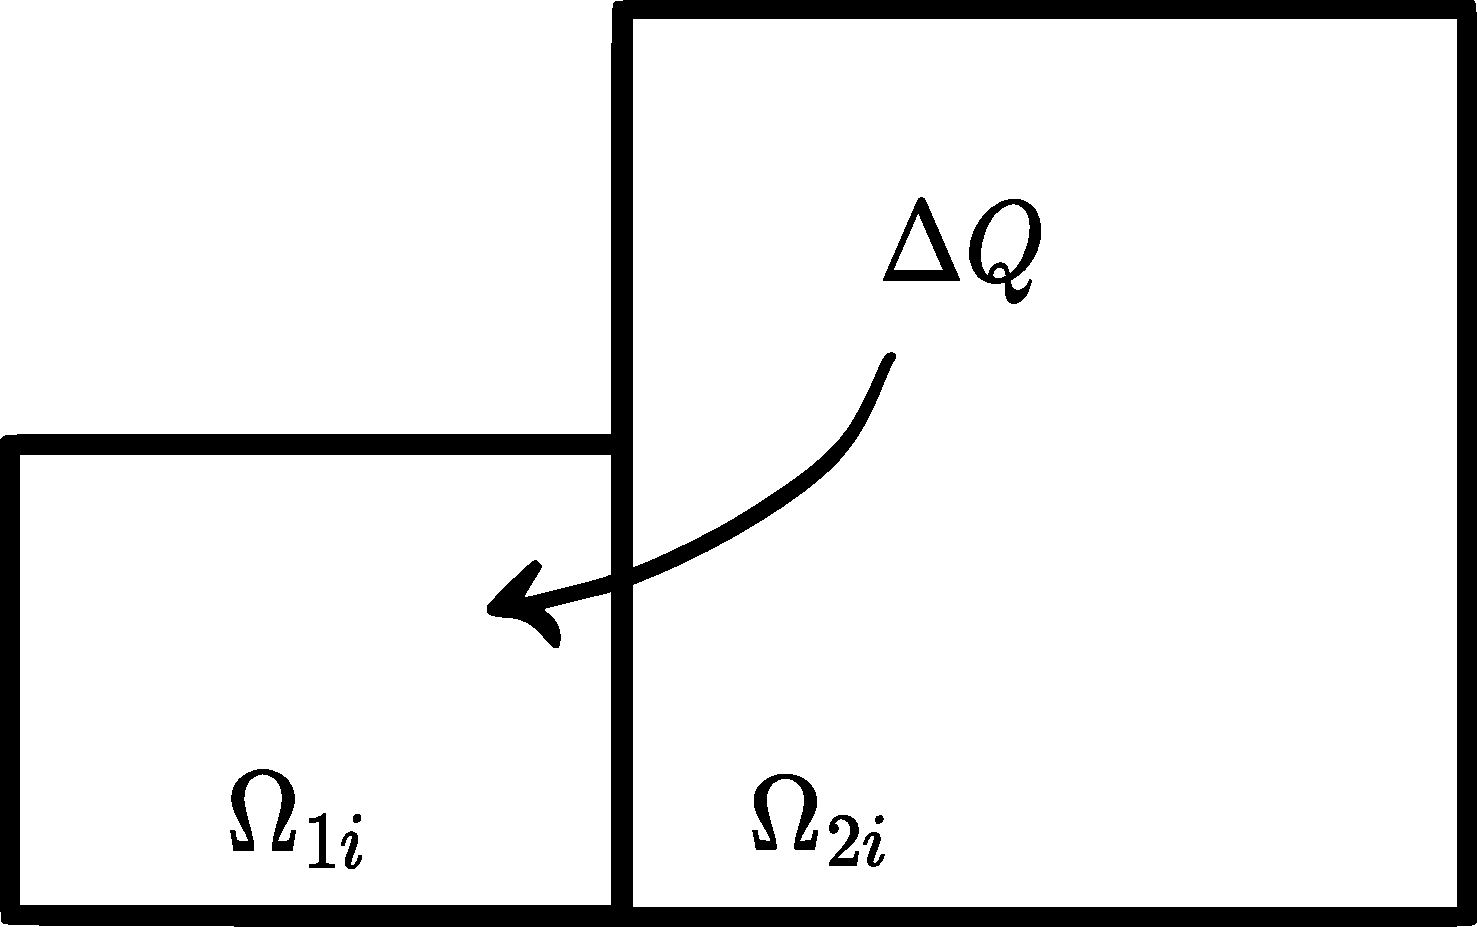
\includegraphics[scale=0.25]{fig/transf-calor.pdf}
\end{figure}

entonces hay $\Omega_{\text{tot},i}=\Omega_{1i}\cdot \Omega_{2i}$ estados accesibles al sistema combinado. Luego, la transferencia de calor ($\Delta Q$) hay $\Omega_{tot,f}=\Omega_{if}\cdot \Omega_{2f}$ estados accesibles al sistema combinado
\begin{equation}
  \Omega_{tot,f}>\Omega_{tot,i}
\end{equation}
En términos de la entropia:
\begin{equation}
  S_{1i}=k\log \Omega_{1i},\qquad  S_{2i}=k\log \Omega_{2i}
\end{equation}
Luego,
\begin{align}
  S_{tot,i}&=k\log \Omega_{tot,i}\\
  &=k\log (\Omega_{1i}\cdot \Omega_{2i})\\
  &=k\log (\Omega_{1i})+k\log (\Omega_{2i})
\end{align}
Así,
\begin{equation}
  S_{tot,i}=S_{1i}+S_{2i}
\end{equation}
Se concluye que la entropía es extensiva.

Notemos ademas que
\begin{equation}
  \Omega_{tot,f}>\Omega_{tot,i}\quad \Rightarrow \quad S_{tot,f}>S_{tot,i}
\end{equation}
es decir, la entropía aumenta en un proceso  de transferencia de calor.
\end{ej}

¿Cuál es la condición de equilibrio para que termine un proceso de transferencia de calor?

Cuando ambos sistemas quedan a la misma \textbf{temperatura}. Para definir temperatura, consideremos que en el nuevo equilibrio térmico:
\begin{equation}
  \left(\pdv{S_1}{U}\right)_{N,V}=-\left(\pdv{S_2}{U}\right)_{N,V}
\end{equation}
\begin{itemize}
	\item La energía interna $U$ cambia en ambos sistemas
	\item La ganancia $\Delta U_1$ en el sistema 1 es igual a la perdida $\Delta U_2$ en el sistema 2 (conservación de la energía).
	\begin{equation}
  \Delta U_1+\Delta U_2=0
\end{equation}
\item La entropía total aumenta, al cambiar $U$. Luego, $\Delta U$ deja de fluir cuando $S_{tot}$ deja de cambiar.
\item Se puede demostrar que el proceso continua hasta que (de lo anterior)
\begin{equation}
	\boxed{\left(\pdv{S_1}{U}\right)_{N,V}=-\left(\pdv{S_2}{U}\right)_{N,V}}
\end{equation}
\end{itemize}

Cuando
\begin{equation}
  \left(\pdv{S_1}{U}\right)_{N,V}=-\left(\pdv{S_2}{U}\right)_{N,V}
\end{equation}
entonces
\begin{equation}
  \left(\pdv{S_{tot}}{U}\right)_{N,V}=\left(\pdv{(S_1+S_2)}{U}\right)_{N,V}=\left(\pdv{S_1}{U}\right)_{N,V}+\left(\pdv{S_2}{U}\right)_{N,V}=0
\end{equation}
Luego,
\begin{equation}
\boxed{  \left(\pdv{S_{tot}}{U}\right)_{N,V}=0}
\end{equation}
y la entropía deja de aumentar con la transferencia de calor. Luego, el proceso se detiene. Así, conviene definir la temperatura $T$:
\begin{equation}
  \boxed{\frac{1}{T}=\left(\pdv{S}{U}\right)_{N,V}}\qquad \text{Al aumentar $T$ aumenta $U$.}
\end{equation}
Notamos que
\begin{equation}
  T_1=T_2\quad\Rightarrow\quad \frac{1}{T_1}=\frac{1}{T_2}\quad\Rightarrow \quad\left(\pdv{S_1}{U}\right)_{N,V}=\left(\pdv{S_2}{U}\right)_{N,V}
\end{equation}

\begin{cor}
	La transferencia de calor ocurre por gradiente de temperatura (el calor fluye desde e sistema de mayor temperatura hacia el de menor temperatura, asta que las temperaturas sean iguales).
\end{cor}

\subsection{Probabilidad de una configuración y factor de Boltzmann}
De la definición clásica de probabilidad, se tiene
\begin{equation}
  P=\frac{\# \text{casos favorables}}{\# \text{casos posibles}}
\end{equation}
El cuociente entre la probabilidad de dos estados macroscópicos es igual al cociente de sus \textit{degeneraciones.}

Considere un sistema \textit{pequeño} de 2 estados, $S_p$ y un sistema \textit{grande} o reservorio térmico $S_r$. Sea $U_0$ la energía del sistema combinado y $U_p$ la energía del sistema pequeño. Suponga que la energía del sistema $U_p$ puede ser $U_p=\epsilon$ y $U_p=0$.
\begin{itemize}
	\item Para $U_p=0$,\quad $U_r=U_0$\quad ($U_r$ energía del reservorio térmico)
	\item Para $U_p=\epsilon$,\quad $U_r=U_0-\epsilon$
\end{itemize}
El cociente entre las probabilidades esta dado por
\begin{equation}\label{1.1}
  \frac{P(\epsilon)}{P(0)}=\frac{\Omega(U_0-\epsilon)}{\Omega(U_0)}=\frac{e^{\frac{S}{k}(U_0-\epsilon)}}{e^{\frac{S}{k}(U_0)}}=\frac{\text{Prob. del $S_p$ con energía $\epsilon$}}{\text{Prob. del $S_p$ con energía $0$}}
\end{equation}
Luego, $\Omega(U)$ es la degeneración del reservorio térmico con energía $U$.

Expandiendo en serie de Taylor 
\begin{equation}
  S(U_0-\epsilon)\approx S(U_0)-\epsilon\left(\pdv{S}{U_0}\right)=S(U_0)-\frac{\epsilon}{T}
\end{equation}
Reemplazando en la exponencial de \eqref{1.1},
\begin{equation}
  \boxed{\frac{P(\epsilon)}{P(0)}\approx e^{-\frac{\epsilon}{kT}}}
\end{equation}
Conocido como el \textbf{factor de Boltzmann}.

La probabilidad relativa entre 2 estados escala como la exponencial de menos la diferencia de energía dividida por $kT$.

\begin{equation}
  	\textbf{Mientras más energético un estado, menos probable.}
\end{equation}

































\newpage
\section{Clase 2}\label{clase:2}
\subsection{Entropía, ignorancia y teorema ergódico}
\begin{tcolorbox}
	\textbf{Principio de máxima entropía}: La configuración de un sistema desde el punto de vista macroscópico, es tal que maximiza la entropía, dada una serie de restricciones.
\end{tcolorbox}

Considere un número grande de sistemas idéntcos ($N_s\to \infty$), cada uno de los cuales puede estar en un estado específico.

Sea $n_i$ el número de sistemas que están en el estado $i$. Definimos la ignorancia $I$ (o la degeneración $\Omega$) como el número de formas de arreglar el sistema conjunto dado $\{n_i\}$ (factor multinomial)
\begin{equation}
  \boxed{I=\frac{N_s!}{n_0!n_1!\cdots},\qquad \sum_i n_i=N_s}
\end{equation}
\begin{ej}
	10 dados, cada uno puede estar en 6 estados. Luego, de tirarlos se obtiene que
	\begin{align}
  n_1&=4\\
  n_2&=3\\
  n_3&=0\\
  n_4&=0\\
  n_5&=0\\
  n_6&=3
\end{align}
entonces la configuración del sistema dada esta ignorancia es
\begin{equation}
  I=\frac{10!}{4!3!3!}
\end{equation}
\end{ej}
Esta ignorancia considera que sólo se conocen las poblaciones de los estados (cuantos sistemas hay en cada estado) y el número total de sistemas, pero que \textit{no es posible distinguir} entre sistemas que están en un mismo estado.

Buscamos una configuración (conjunto de poblaciones de estados) que maximice la ignorancia, sujeto a la restricción
\begin{equation}\label{2.1}
  \sum _i n_i=N_s
\end{equation}
Definimos\footnote{Cantidad extensiva. Maximizar $I$ implica maximizar $S$ (ya que el $\ln$ es monótono.) $\ln I \uparrow=S\uparrow$}
\begin{equation}
  \boxed{S=k\ln I}
\end{equation}
Entonces \begin{equation}\label{2.S}
  S=k\ln\left(\frac{N_s!}{n_0!n_i\cdots}\right)=k[\ln(Ns!)-\sum_i\ln(n_i!)]
\end{equation}
sujeto a \eqref{2.1}.

\textbf{Aproximación de Stirling:}
\begin{equation}\label{Stearling}
  \boxed{\ln(n!)\approx n\ln(n)-n}
\end{equation}

En efecto,
\begin{align}
  \ln(n!)=\ln(1\cdot 2\cdots n)&=\sum_i^n\ln(i)\approx\int_1^n\ln(x)\dd x\\
  &=\eval{x\ln x-x}_1^n\\
  &=(n\ln n-n)-(\cancelto{0}{\ln(1)}-1)\\
  &=n\ln n-n+1\\
  &=n\ln n-(n-1)\\
  &\approx n\ln n-n,\qquad \text{para $n\gg 1$}
\end{align}
Usando la aproximación de Sterling en \eqref{2.S}
\begin{align}
  S&\approx k\left[(N_s\ln(N_s)-\cancel{N_s})-\sum_i (n_i\ln(n_i)-\cancel{n_i})\right]\\
  &=k\left[N_s\ln(N_s)-\sum_in_i\ln(n_i)\right]
\end{align}
donde usamos que $N_s=\sum_i n_i$.

Dado $N_s$ fijo, buscamos $\{n_i\}$ que maximice $S$ sujeto a \eqref{2.1}. Como queremos maximizar utilizamos \textbf{multiplicadores de Lagrange}\footnote{Recordar que para una restricción holonómica $f(\{n_i\})=0$ se incluye $\lambda f$.}.
\begin{equation}
  S_{\{\sum_in_i=N\}}=k\left[N_s\ln(N_s)-\sum_in_i\ln(n_i)+\lambda \left(\sum_in_i-N_s\right)\right]
\end{equation}
Ahora
\begin{equation}
  L=\frac{S}{N_sk},\qquad \mu=\frac{\lambda}{k}
\end{equation}
Nos queda 
\begin{equation}
  L=\ln(N_s)-\sum_i\left(\frac{n_i}{N_s}\right)\ln(n_i)+\mu\left[\sum_i\left(\frac{n_i}{N_s}\right)-1\right]
\end{equation}
Definimos la probabilidad de que en la configuración total, un sistema cualquiera este en el estado $i$ como
\begin{equation}\label{sum Pi1}
  P_i=\frac{n_i}{N_s}
\end{equation}
Reescribimos
\begin{equation}
  \ln(n_i)=\ln\left(\frac{n_i}{N_s}N_s\right)=\ln(P_i)+\ln(N_s)
\end{equation}
Reemplazamos
\begin{align}
  L&=\ln(N_s)-\sum_i P_i\left(\ln(P_i)+\ln(N_s)\right)+\mu\left[\sum_i P_i-1\right]\\
  &=\ln(N_s)-\sum_iP_i\ln(P_i)-\sum_i P_i\ln(N_s)+\mu\left[\sum_i P_i-1\right],\qquad \sum_iP_i=1\\
  &=\cancel{\ln(N_s)}-\sum_iP_i\ln(P_i)-\cancel{\ln(N_s)}+\mu\left[\sum_iP_i-1\right]
\end{align}
Nos queda
\begin{equation}\label{2.2}
  L=-\sum_iP_i\ln(P_i)+\mu\left[\sum_i P_i-1\right]
\end{equation}
Las variables dinámicas son $\{P_i,\lambda\}$. Maximizando $L$
\begin{align}
  \pdv{L}{P_i}&=0\\
  \pdv{L}{\mu}&=0
\end{align}
Ahora, de \eqref{2.2},
\begin{align}
  \pdv{L}{P_i}&=-(\ln P_i+1)+\mu =0\label{2.3} \\
  \pdv{L}{\mu}&=\sum_i P_i=1
\end{align}
donde $\mu$ es constante. De \eqref{2.3},
\begin{equation}
  P_i=e^{\mu-1}=P,\qquad \sum_i P =1
\end{equation}
es decir, \corr{en la configuración que maximiza la entropía, cada estado es igualmente probable} (la probabilidad es igual a una constante que no depende de $i$).

Hay $s$ estados posibles, luego
\begin{equation}
  sP=1\quad \Rightarrow \qquad P=\frac{1}{s}
\end{equation}

Esto implica que la probabilidad de cada estado en la configuración de máxima entropía es
\begin{equation}
  \frac{1}{\# \text{ estados posibles}}
\end{equation}
luego,
\begin{equation}
  \boxed{n_i=N_sP=\frac{N_s}{s}},\qquad \Rightarrow \qquad \sum_{i=1}^sn_i=N_s
\end{equation}
La ocupación de cada estado, en la configuración que maximiza la entropía (y que maximiza la ignorancia o degeneración) es igual al número de sistemas presentes dividido en el número de estados posibles. 













































\newpage
\section{Clase 3}\label{clase:3}
\subsection{Principio fundamental de la termodinámica}
\begin{tcolorbox}
La configuración total \textbf{maximiza la entropía}, sujeta a restricciones macroscópicas que dependen de las cantidades fluctuantes conservadas.
\end{tcolorbox}

En la Clase \ref{clase:2} vimos que si suponemos una configuración $N_s$ sistemas los que pueden existir en $m$ estados diferentes, siendo sus ocupaciones el conjunto:
\begin{equation}
  \{n_i\}_{i=1}^m
\end{equation}
la ignorancia $I$, o degenerancia $\Omega$ esta dada por
\begin{equation}
  \boxed{I=\frac{N_s!}{\Pi_{i=1}^mn_i}}
\end{equation}
Se define la entropía $S$ como
\begin{equation}
  \boxed{S=\kappa \ln I}
\end{equation}
Usando Stearling, se tiene
\begin{align}
  \frac{S}{\kappa}=N_s\ln (Ns)-Ns-\left[\sum_{i=1}^m\left(n_i\ln (n_i)-n_i\right)\right]
\end{align}
Usando que $\sum_{i=1}^m=N_s$,
\begin{align}
  \frac{S}{\kappa}&=N_s\ln (Ns)-\summ n_i\ln(n_i)\quad /\frac{1}{N_s}\\
  \frac{S}{\kappa N_s}&=\ln(N_s)-\summ\left(\frac{n_i}{N_s}\right)\ln (n_i)\label{3.1si}
\end{align}
Usando que
\begin{equation}
  \ln(n_i)=\ln\left(\frac{n_i}{N_s}N_s\right)=\ln\left(\frac{n_i}{N_s}\right)+\ln(N_s)
\end{equation}
reemplazando en \eqref{3.1si},
\begin{align}
  \frac{S}{\kappa N_s}&=\ln (N_s)-\summ\left(\frac{n_i}{N_s}\right)\left[\ln(\frac{n_i}{N_s})+\ln (N_s)\right]\\
  &=\ln(N_s)-\summ \left(\frac{n_i}{N_s}\right)\ln(\frac{n_i}{N_s})-\summ \left(\frac{n_i}{N_s}\right)\ln(N_s)
\end{align}
pero usando \eqref{sum Pi1}
\begin{equation}
  \summ \left(\frac{n_i}{N_s}\right)=\summ P_i=1
\end{equation}
así,
\begin{align}
  \frac{S}{\kappa N_s}&=\ln(N_s)-\summ \left(\frac{n_i}{N_s}\right)\ln(\frac{n_i}{N_s})-\ln(N_s)\\
  &=-\summ\left(\frac{n_i}{N_s}\right)\ln(\frac{n_i}{N_s})
\end{align}
\begin{equation}
  \Rightarrow \boxed{\frac{S}{\kappa N_s}=-\summ\left(\frac{n_i}{N_s}\right)\ln(\frac{n_i}{N_s})}
\end{equation}
Definimos la probabilidad de que un sistema esté en el estado $i$ como \eqref{sum Pi1}
\begin{equation}
\boxed{P_i=\frac{n_i}{N_s}}
\end{equation}
y la entropia de Shannon como
\begin{equation}
  \boxed{\frac{S}{\kappa N_s}=-\summ P_i\ln (P_i)}
\end{equation}
Por el principio fundamental del termodinámica, sin imponer conservación de las cantidades conservadas. Pero considerando
\begin{equation}
  \summ P_i=1
\end{equation}
maximizamos la entropía
\begin{align}
  L&=-\summ P_i\ln(P_i)+\lambda\left(\summ P_i-1\right)
\end{align}
donde $\lambda$ son los multiplicadores de Lagrange y $\summ P_i-1$ es una restricción holonómica.
\begin{align}
  \left(\pdv{L}{P_i}\right)_{P_i,\lambda}&=0,\qquad \forall i\neq j\label{3.1}\\
  \left(\pdv{L}{\lambda}\right)_{P_i}&=0\label{3.2}
\end{align}
De \eqref{3.1}
\begin{align}
  -\ln(P_i)-P_i\frac{1}{P_i}+\lambda&=0\\
  \Rightarrow \ln(P_i)&=\lambda-1
\end{align}
obtenemos
\begin{equation}
  P_i=e^{\lambda-1}
\end{equation}
notemos que esta expresión es independiente de $i$.
De \eqref{3.2},
\begin{align}
  \summ P_i-1&=0\\
 \Rightarrow \summ P_i&=1\\
 \Rightarrow \summ P_i&=mP=me^{\lambda-1}=1
\end{align}
luego
\begin{equation}
  P_i=\frac{1}{m}\quad \Rightarrow\quad n_i=\frac{N_s}{m}\quad\Rightarrow\quad \lambda=-\ln(n)+1
\end{equation}
\corr{Sin imponer restricciones de conservación, excepto que la suma de las probabilidades de los estados es igual a $1$, obtenemos que la configuración que maximiza la entropía es la distribución uniforme de estados equiprobables}. La ocupación de cada uno de los $m$ estados es:
\begin{equation}
  \boxed{n_i=\frac{N_s}{m}}
\end{equation}

\bako{Si imponemos conservación de la energía},
\begin{itemize}
	\item Cada estado $i$ tiene energía $E_i$
	\item Si las ocupaciones de dichos estados son $n_i$, la energía total de la configuración es
	\begin{equation}
  E=\summ E_in_i
\end{equation}
\item Agregamos la conservación de $E$ como una restricción al funcional de entropía.
\end{itemize}

Sea $S_E$ la restricción
\begin{equation}
  S_E=\b \k \left(E-\summ E_in_i\right)
\end{equation}
con $\b$ un multiplicador de Lagrange. Consideremos
\begin{equation}
  L_E=\frac{S_E}{\k N_s}=\b \left(\bar{E}-\summ E_iP_i\right)
\end{equation}
donde 
\begin{equation}
  \bar{E}=\frac{E}{N_s}
\end{equation}
es la energía promedio del sistema.

Luego, nuestro Lagrangeano queda
\begin{equation}
  L=-\summ P_i\ln(P_i)-\lambda \left(\summ P_i-1\right)-\b \left(\summ E_iP_i-\bar{E}\right)
\end{equation}
Ahora,
\begin{align}
  \left(\pdv{L}{P_i}\right)_{P_i,\lambda}&=\ln(P_i)-1-\lambda-\b E_i\\
  \left(\pdv{L}{\b}\right)_{P_i,\lambda}&=\summ E_iP_i=\bar{E}\\
  \left(\pdv{L}{\lambda}\right)_{P_i,\b}&=\summ P_i=1
\end{align}
\begin{equation}
  \ln(P_i)=-\lambda-\b E_i-1
\end{equation}
entonces
\begin{equation}
\boxed{  P_i=e^{-\lambda-\b E_i-1}}
\end{equation}
\begin{align}
  P_i&=e^{-\lambda-1}e^{\b E_i}\\
  \summ P_i&=1\Rightarrow \summ e^{-\lambda-1}e^{-\b E_i}=1\\
  \Rightarrow (e^{-\lambda-1})\summ e^{\b E_i}=1\\
  \Rightarrow e^{-\lambda-1}&=\frac{1}{\summ e^{-\b E_i}}
\end{align}
tenemos
\begin{equation}
  \boxed{P_i=\frac{e^{-\b E_i}}{\summ e^{-\b E_i}}}\quad \Rightarrow\quad \boxed{z=\summ e^{-\b E_i}}\quad \Rightarrow\quad \boxed{P_i=\frac{e^{-\b E_i}}{z}}
\end{equation}
En el caso de imponer conservación de la energía, la configuración solo puede explorar conjuntos de ocupaciones $\{n_i\}_{i=1}^n$ que tengan la misma energía total.

En general, la configuración equiporbable no es alcanzable necesariamente, ya que tiene una energá total particular, que puede ser diferente a la energía inicial dada.

En particular, la energía de la configuración equiprobable es
\begin{align}
  E_{\rm equi}&=\summ E_in_i\\
  &=\summ E_i\frac{N_s}{n}
\end{align}
esto implica
\begin{equation}
  \boxed{E_{\rm equi}=\frac{N_s}{n}\summ E_i}
\end{equation}
Si $E\neq E_{\rm equi}$, la configuración equiprobable es inalcanzable. Para $E$ consevado, la probabilidad de que un sistema esté en el estado $i$ es
\begin{equation}
 \boxed{P_i=\frac{e^{-\b E_i}}{z}}
\end{equation}
donde
\begin{equation}
\boxed{  z=\summ e^{-\b E_i}}
\end{equation}
se conoce como la \textbf{función de partición} y $e^{-\b E_i}$ se llama \textbf{factor de Boltzmann} y tiene la interpretación de un peso estadistico.
\begin{itemize}
	\item $z$ es la suma de todos los pesos
	\item La ocupación del estado $i$ es
	\begin{equation}
\boxed{  n_i=N_sP_i=N_s\frac{e^{-\b E_i}}{z}}
\end{equation}
\end{itemize}

\subsection{Conservación de energía y carga $Q$}
$Q$ puede ser número de partículas, carga eléctrica, momento angular, magnetización, etc...

$Q$ es una cantidad macroscópica, extensiva, diferente de $(E,V,S)$ que caracteriza la configuración macroscópica y que se conserva entre las distintas configuraciones.

El Lagrangeano se verá
\begin{equation}
  L=-\summ P_i\ln(P_i)-\underbrace{\lambda \left(\summ P_i-1\right)}_{\summ P_i=1}-\underbrace{\b\left(\summ E_iP_i-\bar{E}\right)}_{\text{Conservación de la energía}}-\underbrace{\b \m\left(\summ Q_iP_i-\bar{Q}\right)}_{\text{Conservación de la carga}}
\end{equation}
con $\bar{Q}$ la carga promedio del sistema.

Ahora
\begin{align}
  -\ln(P_i)-1-\lambda-\b E_i-\b\m Q_i&=0\\
  P_i=e^{\lambda-1-\b E_i-\b\m Q_i}&=0\\
  P_i&=e^{-\lambda-1}e^{-\b(E_i+\m Q_i)}
\end{align}
usando $\summ P_i=1$,
\begin{align}
  \summ e^{-\b (E_i+\m Q_i)}=\frac{1}{e^{-\lambda-1}}
\end{align}
Definimos
\begin{equation}
\boxed{  Z_{\rm GC}=\summ e^{-\b (E_i+\m Q_i)}}
\end{equation}
entonces
\begin{equation}
 \boxed{ P_i=\frac{e^{-\b (E_i+\m Q_i)}}{Z_{\rm GC}}}
\end{equation}
donde $Z_{\rm GC}$ es la \textbf{función partición Gran Canónica} y corresponde a la suma de los pesos estadisticos $e^{-\b (E_i+\m Q_i)}$. $n_i=N_sP_i$ es la ocupación de los estados.

\subsection{Ensambles, funciones de partición y potenciales termodinámicos}
\begin{itemize}
	\item Maximizando la entropía, sujeto a diferentes restricciones, hemos encontrado la probabilidad de ocupación de los estados posibles de los sistemas.
	\item Dichas probabilidades pueden interprearse como pesos estadisticos para cada estado, normalizados por una función partición.
	\item Dependiendo de las cantidades conservadas las funciones partición son ditintas.
	\item El conjunto de configuraciones posibles dadas las restricciones, definen la noción de ensamble.
	\item A cada tipo de ensamble, especificado por ciertas cantidades conservadas, le corresponde una función partición.
\end{itemize}


\begin{center}
\begin{tabular}{|c|c|c|c|c|}
\hline
  Ensamble & Can. fluctuantes conservadas & Can. fijas & Función partición & Pot. termodinámico  \\
  \hline\hline
  Microcanónico & ----- & $E,V,Q$& $I$& $S$ \\\hline
  Canónico&$E$ &$T,V,Q$&$z=\summ e^{-\b E_i}$&$F$\\\hline
  Gran Canónico&$E,Q$&$T,V,\m$&$z=\summ e^{-\b(E_i+\m Q_i)}$&$\Omega_{\rm GC}$\\\hline
  Isobárico&$E,V$&$T,P,Q$&&\\\hline
\end{tabular}
\end{center}
donde
\begin{equation}
  \b=\frac{1}{T}
\end{equation}

Notas que $\b,\m$ y $P$ son intensivas.

$T=\frac{1}{\b}$ viene dado por el multiplicador de Lagrange asociado a la conservación de energía.






































\newpage
\section{Clase 4}
\subsection{Ensamble micro-canónico}
De la Clase \ref{clase:3} vimos que en el ensamble micro-canónico
\begin{equation}
  P_i=\frac{n}{N_s}
\end{equation}
cada estado equiprobable. $(E,V,Q)$ están fijos.

\subsection{Ensamble canónico}
%En el \textbf{ensamble canónico},
\begin{align}
  P_i&=\frac{1}{Z_{\rm C}}e^{-\b E_i}\\ Z_{\rm C}&=\summ e^{-\b E_i}\\ \bar{E}&=\summ P_iE_i \quad \text{(restricción)}\\
  \b&=\frac{1}{T}
\end{align}
$(T,V,Q)$ están fijos. $\bar{E}$ es fluctuante.

\subsection{Ensamble Gran Canónico}
%En el \textbf{ensamble Gran Canónico},
\begin{align}
  P_i&=\frac{1}{Z_{\rm GC}}e^{-\b E_i-\a Q_i}\\
  Z_{\rm GC}&=\summ e^{-\b E_i-\a Q_i}\\
  \bar{E}&=\summ P_iE_i\label{4.1}\\
  \bar{Q}&=\summ P_iQ_i\label{4.2}\\
  \b&=\frac{1}{\k T}\\
  \a&=-\frac{\m}{\k T}
\end{align}
Aquí \eqref{4.1} y \eqref{4.2} son restricciones. $(T,V,\m)$ están fijos. $\bar{E}$ y $\bar{Q}$ son fluctuantes.

La configuración de cada ensamble \textbf{maximiza la entropía} sujeta a las restricciones correspondientes, implementadas mediante multiplicadores de Lagrange.

\begin{tcolorbox}
	A partir de ahora introduciremos la siguiente \textbf{notación}, 
	\begin{itemize}
		\item $T$: temperatura
		\item $\m$: potencial químico
		\item $z$: función partición
		\item $\k$: Constante de Boltzmann
	\end{itemize}	
\end{tcolorbox}

Partiendo de la función partición (considerando el ensamble Gran Canónico por generalidad), se tiene
\begin{align}
  \bar{E}&=\summ P_iE_i=\frac{\summ E_ie^{-\b E_i-\a Q_i}}{Z}\\
  &=-\left(\pdv{\b}\ln(Z)\right)_\a\label{E=partial-beta}
\end{align}
\begin{equation}
\boxed{  \bar{E}=\k T^2\left(\pdv{T}\ln(Z)\right)_{\m/T}}
\end{equation}
con \begin{equation}
  \b =\frac{1}{\k T}\quad \Rightarrow\quad \pdv{\b }=-T^2\kappa\pdv{T}
\end{equation}
también tenemos
\begin{align}
  \bar{Q}&=\frac{\summ Q_ie^{-\b E_i-\a Q_i}}{Z}\\
  &=-\left(\pdv{\a }\ln(Z)\right)_\b 
\end{align}
\begin{equation}
 \boxed{ \bar{Q}=\k T\left(\pdv{\m }\ln(Z)\right)_T}
\end{equation}
con
\begin{equation}
  \a =\frac{\m }{\k T}\quad \Rightarrow\quad \pdv{\a }=\k T\pdv{\m }
\end{equation}
También es posible relacionar la función partición con la entropía
\begin{align}
  S&=-\k \summ P_i\ln(P_i)\\
  &=\k\summ P_i(\ln(Z)+\b E_i+\a Q_i)\\
  &=\k \left(\ln(Z)+\b \bar{E}+\a \bar{Q}\right)
\end{align}
luego
\begin{equation}
\boxed{  S=\k \ln(z)+\frac{\bar{E}}{T}-\frac{\m \bar{Q}}{T}}\quad \Rightarrow\quad \boxed{-\k T\ln(z)=\bar{E}-TS-\m Q}
\end{equation}

Para los diferentes ensambles, existen potenciales termodinámicos definidos en términos de $\ln(Z)$. \footnote{Los signos y los factores delante son por razones históricas, desafortunadamente. :(}

\textbf{Potencial Gran Canónico}
\begin{equation}
  \Omega_{\rm GC}=-\k T\ln(Z_{\rm GC})=\bar{E}-TS-\m\bar{Q}
\end{equation}

\textbf{Energía libre de Hemholtz}
\begin{equation}
  F=-\k T\ln(Z_{\rm C})=\bar{E}-TS\quad (Q_i=0)
\end{equation}

Existen relaciones entre los potenciales termodinámicos de los diferentes ensambles. Por ejemplo, definiendo la \textbf{densidad de estados}
\begin{equation}
  \r(Q,E)=\frac{e^{S(Q,E)/\kappa}}{\delta E}	
\end{equation}
$\r(Q,E)$ cuenta el número de estados con carga $Q$ y energía entre $E$ y $E+\delta E$. De aquí podemos obtener la energía libre de Hemholtz como
\begin{equation}
  F(Q,T)=-\k T\ln(Z_{\rm C})=-\k T\ln\int\dd E\r(Q,E)e^{-E/\k T}
\end{equation}
Finalmente el potencial Gran Canónico, puede calcularse como
\begin{equation}
  \Omega_{\rm GC}(\m,T)=\k T\ln(\zgc)=-T\ln\left(\sum_Qe^{-F(Q,T)/\k T}e^{\m Q/\k T}\right)
\end{equation}

\subsection{Ensamble isobárico-isotérmico}
En el ensamble isobárico-isotérmico $(T,P,Q)$ son constantes y $(\bar{E},\bar{V})$ son fluctuantes.

Notemos que $V$ es una cantidad extensiva (proporcional al número total de sistemas $N_s$). Si no hay restricciones entre sistemas, el potencial Gran Canónico por unidad de volumen es independiente del volumen (cada región es igual a cualquier otra).

Por último, la presión se define como menos la derivada del potencial termodinámico (Gran Canónico) con respecto al volumen. Luego,
\begin{equation}
  \Omega_{\rm GC}=\o_{\rm GC}V
\end{equation}
donde $\o_{\rm GC}$ es el potencial Gran Canónico por unidad de volumen. Se sigue que
\begin{equation}
  \pdv{\ogc}{V}=0
\end{equation}
así,
\begin{equation}
  P=\pdv{V}\Ogc=-\ogc=-\frac{\Ogc}{V}
\end{equation}
Entonces
\begin{equation}
\boxed{  \Ogc=-PV=-\k T\ln(\zgc)=E-TS-\m Q}
\end{equation}
\begin{equation}\label{4.3}
\boxed{  PV=TS-E+\m Q}
\end{equation}
Se define $G$, la \textbf{enegía libre de Gibbs}, como\footnote{se deriva de \eqref{4.3}}
\begin{equation}
\boxed{  G=\m Q=E-TS+PV}
\end{equation}

$G$ es el potencial termodinámico del ensamble isobárico-isotérmico.

Además, podemos obtener la siguiente relación
\begin{equation}
\boxed{  E=TS-PV+\m Q}
\end{equation}
conocida como la \textbf{relación de Euler}.






















\newpage
\section{Clase 5}
\subsection{Relaciones termodinámicas}
Hasta el momento hemos obtenido las siguientes relaciones termodinámicas
\begin{tcolorbox}
\begin{itemize}
	\item Relación de Euler
	\begin{equation}
  E=TS-PV+\m Q
\end{equation}
\item Energía libre de Hemholtz \begin{equation}
  F=-\k T\ln(\zc)=E-TS
\end{equation}
\item Potencial gran canónico
\begin{equation}\label{5.star}
  \Ogc=-PV=-\k T\ln (\zgc)=E-TS-\m Q
\end{equation}
\item Energía libre de Gibbs
\begin{equation}
  G=\m Q=E-TS+PV
\end{equation}
\end{itemize}
\end{tcolorbox}

Por otro lado, las funciones de partición de cada ensamble y la relación de $E$ y $Q$ con ellas vienen dadas por\footnote{Notar que no escribimos la barra de promedio en $\bar{E}$ y $\bar{Q}$ ya que se sobreentiende donde corresponde.}
\begin{tcolorbox}
\begin{equation}
  \zc =\summ e^{-\b E_i},\qquad \b =\frac{1}{T}
\end{equation}
\begin{equation}
  \zgc=\summ e^{-\b E_i-\a Q_i},\qquad \a=-\frac{\m }{T}
\end{equation}

\begin{equation}\label{5.box1}
  \bar{E}=\k T^2\left(\pdv{T}\ln(Z)\right)_{\m/T}
\end{equation}

\begin{equation}\label{5.box2}
 \bar{Q}=\k T\left(\pdv{\m }\ln(\zgc)\right)_T
\end{equation}
\end{tcolorbox}

\subsection{Derivación de las leyes de la termodinámica}
De \eqref{5.star}
\begin{equation}
  \Ogc=-PV=-\k T\ln (\zgc)=E-TS-\m Q
\end{equation}
despejando para $S$
\begin{equation}
  S=\k \ln(\zgc(\m /T,T,V))+\frac{E}{T}-\left(\frac{\m }{T}\right)Q
\end{equation}
luego,
\begin{align}\label{5.ds}
  \dd S&=\left(\k\pdv{\ln \zgc}{T}-\frac{E}{T^2}\right)\dd T+\left(\k\pdv{\ln\zgc}{(\m/T)}-Q\right)\dd Q+\k\pdv{\ln\zgc}{V}\dd V+\frac{\dd E}{T}-\frac{\m\dd Q}{T}
\end{align}
pero 
\begin{equation}
  PV= T\ln\zgc \qquad \implies\qquad \ln\zgc=\frac{P}{T}V
\end{equation}
tomando la derivada parcial con respecto a $V$
\begin{equation}
  \pdv{\ln\zgc}{V}=\frac{P}{T}
\end{equation}
reemplazando en \eqref{5.ds},
\begin{align}
  \dd S=\left(\k\pdv{\ln \zgc}{T}-\frac{E}{T^2}\right)\dd T+\left(\k\pdv{\ln\zgc}{(\m/T)}-Q\right)\dd Q+\frac{P}{T}\dd V+\frac{\dd E}{T}-\frac{\m\dd Q}{T}
\end{align}
usando \eqref{5.box1} y \eqref{5.box2} se cancelan los primeros dos términos, obteniendo
\begin{equation}
  \dd S=\frac{P}{T}\dd V+\frac{\dd E}{T}-\frac{\m\dd Q}{T}
\end{equation}
\begin{equation}
 \boxed{ T\dd S=P\dd V+\dd E-\m\dd Q}
\end{equation}
conocida como la \textbf{segunda ley de la termodinámica}.

\subsection{Relaciones de equilibrio termodinámico}
Consideremos dos sistemas $C_1$ y $C_2$, los cuales pueden intercambiar energía y carga, y ademas pueden modificar su volumen. De las leyes de conservación se tiene
\begin{equation}
  \boxed{\dd E_1=-\dd E_2,\qquad \dd Q_1=-\dd Q_2,\qquad \dd V_1=-\dd V_2}
\end{equation}
también se tiene
\begin{equation}
 \boxed{ \dd S_{\rm total}=\dd S_1+\dd S_2}
\end{equation}
Es decir, el cambio en la entropía es la suma de los cambios de la entropía de cada sistema.

Ahora
\begin{equation}
  \boxed{\dd S_i=\frac{P_i}{T_i}\dd V_i+\frac{1}{T_i}\dd E_i-\frac{\m_i}{T_i}\dd Q_i}
\end{equation}
Esto es el cambio de la entropía en cada sistema dado por la segunda ley de la termodinámica. Por lo tanto
\begin{equation}
  \boxed{\dd S_{\rm total}=\dd S_1+\dd S_2=\left(\frac{P_1}{T_1}-\frac{P_2}{T_2}\right)\dd V_1+\left(\frac{1}{T_1}-\frac{1}{T_2}\right)\dd E_1+\left(\frac{\m_1}{T_1}-\frac{\m_2}{T_2}\right)\dd Q_1}
\end{equation}
Pero del principio de la máxima entropía, la configuración maximiza la entropía (sujeto a las restricciones de conservación). Luego, en todo proceso termodinámico, $\dd S_{\rm total}\geq 0$.

La condición de equilibrio termodinámico requiere $\dst=0$. Por lo tanto la condición de equilibrio establece:
\begin{equation}
  \frac{P_1}{T_1}=\frac{P_2}{T_2},\qquad \frac{1}{T_1}=\frac{1}{T_2},\qquad \frac{\m_1}{T_1}=\frac{\m_2}{T_2}
\end{equation}
entonces
\begin{align}
  P_1&=P_2\\
   T_1&=T_2\\
    \m_1&=\m_2
\end{align}
esto implica también que le intercambio de energía interna o calor ($E$) se produce desde el sistema de mayor temperatura hacia el de menor temperatura, el intercambio de cargas ($Q$) ocurre desde el sistema de mayor potencial químico hacia el de menor potencial químico y el cambio de volumen ($V$)  ocurre de modo que el sistema con mayor presión se expande y de menor presión se contrae.

\subsection{Otras relaciones termodinámicas}
Por un lado
\begin{equation}
  E=TS-PV+\m Q
\end{equation}
si derivamos
\begin{equation}
  \dd E=\dd TS+T\dd S-\dd PV-P\dd V+\dd\m Q+\m \dd Q
\end{equation}
además de la segunda ley,
\begin{equation}
  \dd E=T\dd S-P\dd V+\m \dd Q
\end{equation}
reemplazamos $\dd E$ en lo anterior y obtenemos
\begin{equation}
  \boxed{S\dd T-V\dd P+Q\dd\m =0}
\end{equation}

\subsubsection{Acerca de los potenciales termodinámicos}
El potencial gran canónico viene dado por
\begin{equation}
  \Omega=E-\m Q-TS
\end{equation}
derivamos
\begin{equation}
  \dd\Omega=\dd E-\dd\m Q-\m \dd Q-\dd TS-T\dd S
\end{equation}
usando de nuevo la segunda ley
\begin{equation}
  T\dd S=P\dd V+\dd E-\m\dd Q
\end{equation}
y obtenemos
\begin{equation}
 \boxed{ \dd \Omega=-S\dd T-P\dd V-Q\dd\m}
\end{equation}
Notar que el ensamble gran canónico tiene $(T,V,\m )$ dijos y $(E,Q)$ fluctuantes. Luego,
\begin{equation}
  \Omega=\Omega(T,V,\m )
\end{equation}
y
\begin{equation}
  \dd\Omega=\left(\pdv{\Omega}{T}\right)_{V,\m }\dd T+\left(\pdv{\Omega}{V}\right)_{T,\m }\dd V+\left(\pdv{\Omega}{\m }\right)_{T,V }\dd \m 
\end{equation}
Por lo tanto,
\begin{align}
  \left(\pdv{\Omega}{T}\right)_{V,\m }&=-S\\
  \left(\pdv{\Omega}{V}\right)_{T,\m }&=-P\\
  \left(\pdv{\Omega}{\m }\right)_{T,V }&=-Q
\end{align}

Para la energía libre de Hemholtz en su versión integrada viene dada por
\begin{equation}
  F=E-TS
\end{equation}
\begin{equation}
  \dd F=\dd E-\dd TS-T\dd S
\end{equation}
Usando nuevamente la segunda ley, obtenemos
\begin{equation}
  \boxed{\dd F=-P\dd V+\m \dd Q-S\dd T}
\end{equation}
En la definición del ensamble canónico, $(T,V,Q)$ estan fijos, y $E$ fluctua. Luego, $F=F(T,V,Q)$, por lo tanto
\begin{equation}
  \dd F=\left(\pdv{F}{T}\right)_{V,Q}\dd T+\left(\pdv{F}{V}\right)_{T,Q}\dd V+\left(\pdv{F}{Q}\right)_{T,V}\dd Q
\end{equation}
luego,
\begin{align}
  \left(\pdv{F}{T}\right)_{V,Q}&=-S\\
  \left(\pdv{F}{V}\right)_{T,Q}&=\m \\
  \left(\pdv{F}{Q}\right)_{T,V}&=-P
\end{align}

Para la energia libre de Gibbs,
\begin{equation}
  G=E+PV-TS
\end{equation}
\begin{equation}
  \dd G=\dd E+\dd PV+P\dd V-\dd T S-T\dd S
\end{equation}
Haciendo un procedimiento similar al de los casos anteriores, se tiene
\begin{equation}
  \boxed{\dd G=-S\dd T+V\dd P+\m \dd Q}
\end{equation}

en el ensamble isobárico-isotérmico, $(T,P,Q)$ están fijas y $(E,V)$ fluctúa. Luego, $G=G(T,P,Q)$, y por tanto
\begin{equation}
  \dd G=\left(\pdv{G}{T}\right)_{P,Q}\dd T+\left(\pdv{G}{P}\right)_{T,Q}\dd P+\left(\pdv{G}{Q}\right)_{P,T}\dd Q
\end{equation}
por tanto
\begin{align}
  \left(\pdv{G}{T}\right)_{P,Q}&=-S\\
  \left(\pdv{G}{P}\right)_{T,Q}&=V\\
  \left(\pdv{G}{Q}\right)_{P,T}&=\m 
\end{align}

La \textbf{entalpía} se define como
\begin{equation}
  H=E+PV
\end{equation}
entonces 
\begin{equation}
  \dd H=\dd E+\dd PV+P\dd V
\end{equation}
reemplazando $\dd E$ de la segunda ley,
\begin{equation}
  \boxed{\dd H=T\dd S+V\dd P+\m \dd Q}
\end{equation}
Por tanto en el \textbf{ensamble de Joule-Thompson}, del cual la es su potencial termodinámico, tiene $(S,P,Q$ fijos y $V$ fluctuante, es decir, $H=H(S,P,Q)$. Luego,
\begin{equation}
  \dd H=\left(\pdv{H}{S}\right)_{P,Q}\dd S+\left(\pdv{H}{P}\right)_{S,Q}\dd P +\left(\pdv{H}{Q}\right)_{P,S}\dd Q
\end{equation}
Luego, nos queda
\begin{align}
  \left(\pdv{H}{S}\right)_{P,Q}&=T\\
  \left(\pdv{H}{P}\right)_{S,Q}&=V\\
  \left(\pdv{H}{Q}\right)_{P,S}&=\m 
\end{align}

Finalmente, para el ensamble microcanónico, las cantidades fijas son $(E,V,Q)$ y de la segunda ley se tiene
\begin{equation}
  \dd E=T\dd S-P\dd V+\m \dd Q
\end{equation}
Luego, se puede despejar
\begin{equation}
  \dd S=\left(\frac{1}{T}\right)\dd E+\left(\frac{P}{T}\right)\dd V-\left(\frac{\m }{T}\right)\dd Q
\end{equation}
y considerando que a $(E,V,Q)$ fijos, se tiene que $S=S(E,V,Q)$ y 
\begin{equation}
  \dd S=\left(\pdv{S}{E}\right)_{V,Q}\dd E+\left(\pdv{S}{V}\right)_{E,Q}\dd V+\left(\pdv{S}{Q}\right)_{V,E}\dd Q
\end{equation}
se tiene que
\begin{align}
  \left(\pdv{S}{E}\right)_{V,Q}&=\frac{1}{T}\\
  \left(\pdv{S}{V}\right)_{E,Q}&=\frac{P}{T}\\
  \left(\pdv{S}{Q}\right)_{V,E}&=-\frac{\m }{T}
\end{align} 

\subsection{Resumen: ensambles y potenciales termodinámicos}
Como resumen, tenemos la siguiente tabla que relaciona los distintos ensambles con sus potenciales termodinámicos y variables fijas:


\begin{center}
\begin{tabular}{|c|c|c|}
\hline
  Ensamble & Potencial termodinámico & Variabes fijas  \\
  \hline
  Microcanónico &Entropía $(S)$& $(E,V,Q)$ \\\hline
  Canónico&Energía libre de Hemholtz $(F)$ &$(T,V,Q)$\\\hline
  Gran Canónico&Potencial gran canónico $(\Ogc)$&$(T,V,\m )$\\\hline
  Isobárico-Isotérmico&Energía libre de Gibbs $(G)$&$(T,P,Q)$\\\hline
  Joule-Thompson&Entalpía $(H)$&$(S,P,Q)$\\\hline
\end{tabular}
\end{center}












































































\newpage
\section{Clase 6}
%De la clase anterior, tenemos la siguiente tabla resúmen
%
%\begin{center}
%\begin{tabular}{|c|c|c|c|}
%\hline
%  Ensamble & Potencial & Definición &Variación del potencial \\
%  \hline
%  Microcanónico &Entropía $S(E,V,Q)$& $S$ & $\dd S=\frac{1}{T}\dd E+\frac{P}{T}\dd V-\frac{\m }{T}\dd Q$ \\\hline
%  Canónico&Energía libre de Hemholtz $F(T,V,Q)$ &$F=E-TS=\m Q-PV$\\\hline
%  Gran Canónico&Potencial gran canónico $(\Ogc)$&$(T,V,\m )$\\\hline
%  Isobárico-Isotérmico&Energía libre de Gibbs $(G)$&$(T,P,Q)$\\\hline
%  Joule-Thompson&Entalpía $(H)$&$(S,P,Q)$\\\hline
%\end{tabular}
%\end{center}

\subsection{Fuerzas a temperatura finita}
El trabajo por hecho por una fuerza al recorrer una distancia $\dd\vec{x}$, está dado por
\begin{equation}
  W=-\int_{\vec{x}_1}^{\vec{x}_2}\vec{f}\cdot\dd\vec{x}
\end{equation}
Esto es una contribución a la energía del sistema.

Supongamos un movimiento en $\vec{x}$. Luego incluyendo la contribución de $W$ a la energía del sistema, la cual funcionalmente es análoga al termino $-P\dd V$, tenemos
\begin{equation}\label{6.star}
  \dd E=T\dd S-P\dd V+\m\dd Q-f\dd x
\end{equation}
donde $f=|\vec{f}_x|$ es la magnitud de la fuerza.

Ahora, suponamos que el sistema está a $T$ constante. Consideremos $F(T,V,Q)$ y la relacionamos con $f$:
\begin{equation}
  F=E-TS
\end{equation}
\begin{equation}
  \dd F=\dd E-S\dd T-T\dd S
\end{equation}
Considerando \eqref{6.star} se tiene
\begin{equation}
  \dd F=-S\dd T-P\dd V+\m \dd Q-f\dd x
\end{equation}
\begin{equation}
  \implies f\dd x=-\dd F-S\dd t-P\dd V+\m\dd Q
\end{equation}
si consideramos $(T,V,Q)$ fijos, se tiene
\begin{equation}
  f\dd x=-\dd F
\end{equation}
luego,
\begin{equation}
 \boxed{ f=-\eval{\left(\pdv{F}{x}\right)}_{T,V,Q}}
\end{equation}
es decir, la energía libre de Hemholtz $F=E-TS$ juega el rol de potencial.

Notemos que $F$ puede obtenerse directamente de la función partición canónica,
\begin{equation}
  \boxed{F=-\k T\ln (\zc)}
\end{equation}

\begin{ej}
	Un ejemplo estándar consiste en derivar la ley de Hooke para una cadena de $N$ eslabones a temperatura $T$.
\end{ej}

\subsection{Relaciones de Maxwell}
Las relaciones de Maxwell consisten en un conjunto de equivalencias entre derivadas de variables termodinámicas.

Todas las relaciones de Maxwell pueden ser derivadas desde la relación fundamental de la termodinámica,
\begin{equation}
  \dd S=\b\dd E+(\b P)\dd V-(\b\m )\dd Q
\end{equation}
de donde podemos identificar directamente,
\begin{align}
  \b=\eval{\pdv{S}{E}}_{V,Q}\\
  \b P=\eval{\pdv{S}{V}}_{E,Q}\\
  \b\m=-\eval{\pdv{S}{Q}}_{V,E}
\end{align}

\begin{ej}
	Considere
	\begin{equation}
  \dd S=\frac{1}{T}\dd E+\frac{P}{T}\dd V-\frac{\m }{T}\dd Q
\end{equation}
Notamos que para $F(x,y)$ continua y $2$ veces diferenciable, se tiene
\begin{equation}
  \pdv{F}{x}{y}=\pdv{F}{y}{x}
\end{equation}
es decir, sus derivadas conmutan. Luego, por ejemplo
\begin{equation}
  \pdv{S}{E}{V}=\pdv{S}{V}{E}
\end{equation}
\begin{equation}
	\left(\pdv{E}\left(\pdv{S}{V}\right)_{E,Q}\right)_{V,Q}=\left(\pdv{V}\left(\pdv{S}{E}\right)_{V,Q}\right)_{E,Q}
\end{equation}
\begin{equation}
  \implies \boxed{\pdv{E}\left(\frac{P}{T}\right)_{V,Q}=\pdv{V}\left(\frac{1}{T}\right)_{E,Q}}
\end{equation}
\end{ej}
Notar que cada potencial termodinámico depende de tres variables y por lo tanto se pueden escoger tres diferentes relaciones entre dobles derivadas. Luego como son $5$ potenciales termodinámicos diferentes (para cada uno de los $5$ ensambles), tenemos $15$ relaciones diferentes entre sus dobles derivadas. \textbf{Estas son $15$ relaciones de Maxwell.}

\begin{ej}
	Consideremos $G=G(T,P,Q)$, así
	\begin{equation}
  \dd G=-S\dd T+V\dd P+\m \dd Q
\end{equation}
Ahora
\begin{equation}
  \pdv{G}{T}{P}=\pdv{G}{P}{T}
\end{equation}
\begin{equation}
  \left(\pdv{T}\left(\pdv{G}{P}\right)_{T,Q}\right)_{P,Q}=\left(\pdv{P}\left(\pdv{G}{T}\right)_{P,Q}\right)_{T,Q}
\end{equation}
\begin{equation}
  \implies \boxed{\eval{\pdv{T}{V}}_{P,Q}=-\eval{\pdv{S}{P}}_{T,Q}}
\end{equation}
\end{ej}

Consideremos otro ejemplo.
\begin{ej}
	Muestre que 
	\begin{equation}
  \left(\pdv{E}{Q}\right)_{S,P}=\m -P\left(\pdv{\m}{P}\right)_{S,Q}
\end{equation}
Vemos que $V$ no aparece. Luego, despejamos la relación de $V$ de la segunda ley
\begin{equation}
  \dd E=T\dd S-P\dd V+\m\dd Q
\end{equation}
\begin{equation}\label{6.2star}
  \implies \dd V=\frac{T}{P}\dd S+\frac{\m }{P}\dd Q-\frac{1}{P}\dd E
\end{equation}
De aquí podemos considerar, sumando $E/P$ para eliminar la dependencia de $\dd E$,
\begin{equation}\label{6.mio}
  \dd\left(V+\frac{E}{P}\right)=\dd V+\frac{\dd E}{\dd P}+E\dd\left(\frac{1}{P}\right)
\end{equation}
Pasando el último término de \eqref{6.2star} hacia el lado derecho y reemplazando \eqref{6.mio},
\begin{equation}
  \dd\left(V+\frac{E}{P}\right)=\frac{T}{P}\dd S+\frac{\m }{P}\dd Q-E\dd\left(\frac{1}{P}\right)
\end{equation}
Entonces 
\begin{equation}
  \pdv{(V+E/P)}{(1/P)}{Q}=\pdv{(V+E/P)}{Q}{(1/P)}
\end{equation}
Notemos que si y sólo si $(1/P)$ es constante,
\begin{equation}
  \left(\pdv{(1/P)}\left(\pdv{\m }{P}\right)\right)_{S,Q}=\left(\pdv{Q}E\right)_{S,P}
\end{equation}
Usando que
\begin{equation}
  \pdv{(1/P)}=-P^2\pdv{P}
\end{equation}
tenemos
\begin{equation}
  \left(\pdv{E}{Q}\right)_{S,P}=-P^2\left(\pdv{P}\left(\pdv{\m }{P}\right)\right)_{S,Q}
\end{equation}
\begin{equation}
   \left(\pdv{E}{Q}\right)_{S,P}=-P^2\left(-\frac{1}{P^2}\m +\frac{1}{P}\left(\frac{\m }{P}\right)_{S,Q}\right)
\end{equation}
\begin{equation}
  \boxed{ \left(\pdv{E}{Q}\right)_{S,P}=\m -P\left(\pdv{\m }{P}\right)_{S,Q}}
\end{equation}
\end{ej}

\subsection{Fluctuaciones}
De la función de partición es posible obtener momentos de orden superior para las variables termodinámicas \footnote{Los momentos de orden superior se pueden entender como derivadas de orden superior de la función partición con respecto a los multiplicadores de Lagrange.} . Por ejemplo, tenemos
\begin{equation}
  \zc=\sumi e^{-\b E_i}
\end{equation}
y por definición la energía promedio viene dada por
\begin{equation}
  \ev{E}=\sumi E_iP_i
\end{equation}
y
\begin{equation}
  P_i=\frac{e^{-\b E_i}}{\zc}
\end{equation}
por lo tanto, de \eqref{E=partial-beta},
\begin{equation}
  \ev{E}=\frac{\sumi E_i e^{-\b E_i}}{\zc}=-\frac{1}{\zc}\pdv{\zc}{(1/\k T)}
\end{equation}
Entonces
\begin{equation}
  \boxed{\ev{E}=-\pdv{(1/\k T)}\ln (\zc)=\k T^2\pdv{T}\ln (\zc)}
\end{equation}
Además,
\begin{equation}
  \ev{E^2}=\sumi E_i^2 P_i=\frac{\sumi E_i^2 e^{-Ei/\k T}}{\zc}
\end{equation}
%Vemos que
%\begin{equation}
%  \boxed{\pdv[2]{\b }\ln (\zc)=(E-\ev{E})^2}
%\end{equation}
%notar que $(E-\bar{E})^2$ es la varianza de $E$. 
Notar que dado que
\begin{equation}
  \beta=\frac{1}{\k T}
\end{equation}
en términos de $\b$ tenemos
\begin{equation}
  \zc=\sumi e^{-\b E_i}
\end{equation}
luego
\begin{align}
  \pdv{\b}\ln (\zc)&=-\frac{1}{\zc}\sumi E_i\eb\\
  &=-\ev{E}
\end{align}
es decir,
\begin{equation}
  \boxed{\pdv{\b}\ln (\zc)=-\ev{E}}
\end{equation}

Calculemos ahora la segunda derivada con respecto a $\b$,
\begin{align}
  \pdv[2]{\b}\ln(\zc)&=\pdv{\b}\left(-\frac{1}{\zc}\sumi E_i\eb\right)\\
  &=\left(\frac{1}{\zc^2}\pdv{\b}\sumi E_i\eb\right)+\frac{1}{\zc}\sumi E_i^2\eb\\
  &=\left(-\frac{1}{\zc^2}E_j\sum_j e^{-\b E_j}\right)\left(\sumi E_i\eb\right)+\frac{1}{\zc}\sumi E_i^2\eb\\
  &=\left(-\frac{1}{\zc}E_j\sum_j e^{-\b E_j}\right)\left(\frac{1}{\zc}\sumi E_i\eb\right)+\frac{1}{\zc}\sumi E_i^2\eb\\
  &=-\ev{E}^2+\ev{E^2}
\end{align}
así,
\begin{equation}\label{6.d2blnz}
 \boxed{ \pdv[2]{\b}\ln(\zc)=\ev{E^2}-\ev{E}^2}
\end{equation}

\begin{prop}
Sea $\ev{E}$ el valor promedio de una cantidad, entonces la varianza de $E$ se puede escribir de dos maneras equivalentes
	\begin{equation}
  \text{Var}({E})=\ev{(E-\ev{E})^2}=\ev{E^2}-\ev{E}^2
\end{equation}
\end{prop}
En efecto,
\begin{align}
  \ev{(E-\ev{E})^2}&=\sumi P_i\left(E_i-\sumj P_j E_j\right)^2\\
  &=\sumi P_i\left(E_i^2-2E_i\sumj P_jE_j+\left(\sumj P_jE_j\right)^2\right)\\
  &=\sumi P_iE_i^2-2\left(\sumi P_iE_i\right)\left(\sumj P_jE_j\right)+\underbrace{\sumi P_i}_{1}\left(\sumj P_jE_j\right)^2\\
  &=\ev{E^2}-2\ev{E}^2+\ev{E}^2\\
  &=\ev{E^2}-\ev{E}^2
\end{align}
Luego, \eqref{6.d2blnz} se puede escribir como
\begin{equation}
  \boxed{\pdv[2]{\b}\ln(\zc)=\ev{(E-\ev{E})^2}\equiv \text{Var}(E)}
\end{equation}

Además, podemos reescribir esto en términos de derivadas de $T$, usando
\begin{equation}
  \b=\frac{1}{\k T}\quad \implies \qquad \pdv{\b}=-\k T^2\pdv{T}
\end{equation}
luego,
\begin{align}
  \pdv{\b}\left(\pdv{\b}\ln\zc\right)&=\pdv{\b}\left(-\k T^2\pdv{T}\ln\zc\right)\\
  &=\k^2 T^2\pdv{T}\left(T^2\pdv{T}\ln\zc\right)\\
  &=\k^2T^2\left(2T\pdv{T}\ln\zc+T^2\pdv[2]{T}\ln\zc\right)
\end{align}
finalmente, se tiene
\begin{equation}
  \boxed{\text{Var}(E)=2\k^2T^3\pdv{T}\ln\zc+\k^2T^4\pdv[2]{T}\ln\zc}
\end{equation}








%\begin{align}
%  \pdv[2]{\b}\ln(\zc)&=-\pdv{\b}\left(\frac{1}{\zc}\sumi E_i\eb \right)\\
%  &=\left(\frac{1}{\zc^2}\sumi E_i\eb\right)\left(\sumi E_i\eb\right)+\frac{1}{\zc}\sumi E_i^2\eb\\
%  &=-\ev{E}^2-\ev{E^2}\\
%  &=\ev{E^2}-\ev{E}^2
%\end{align}
%es decir,
%\begin{equation}
%   \pdv[2]{\b}\ln(\zc)=\ev{E^2}-\ev{E}^2
%\end{equation}
%Luego,
%%TODO checkear
%
%\begin{equation}
%  \ev{(E-\ev{E})^2}=\sumi P_i (E_i-\ev{E})^2=
%\end{equation}

















\newpage
\section{Clase 7}
De la clase anterior se tiene
\begin{equation}
\ev{E}=-\pdv{\b}\ln (\zc)
\end{equation}
\begin{equation}
\text{Var}(E)=\pdv[2]{\b}\ln(\zc)=\ev{(E-\ev{E})^2}=\ev{E^2}-\ev{E}^2
\end{equation}

La función partición también puede relacionarse con la fluctuación de la carga y con la covarianza entre la carga y la energía según
\begin{equation}\label{7.varq}
  \boxed{\var(Q)=\ev{(Q-\ev{Q})^2}=\pdv[2]{\a }\ln\zgc}
\end{equation}
\begin{equation}\label{7.coveq}
  \boxed{\text{Cov}(E,Q)=\ev{(E-\ev{E})(Q-\ev{Q})}=\pdv{\a }\pdv{\b }\ln\zgc}
\end{equation}

En efecto, para \eqref{7.varq} la demostración es análoga al procedimiento que se usó para mostrar \eqref{6.d2blnz} pero ahora considerando $\zgc$.

Para mostrar \eqref{7.coveq}, calculemos la doble derivada de $\ln\zgc$ con respecto a $\a$ y $\b$,
\begin{align*}
 	\partial_\b\partial_\a \ln\zgc&=\partial_\b \left(\frac{1}{\zgc}\partial_\a \left(\sumi \eba\right)\right)\\
 	&=\partial_\b\left(-\frac{1}{\zgc}Q_i\sumi \eba\right)\\
 	&=\left(\frac{1}{\zgc^2}Q_i\partial_\b \zgc\right)\left(\sumi \eba\right)+\frac{1}{\zgc}Q_iE_i\sumi \eba\\
 	&=-\frac{1}{\zgc^2}\left(\sumj E_j\ebaj\right)\left(\sumi Q_i\eba\right)+\frac{1}{\zgc}Q_iE_i\sumi \eba\\
 	&=\ev{EQ}-\ev{E}\ev{Q}
\end{align*}
es decir,
\begin{equation}
  \text{Cov}(E,Q)=\partial_\b\partial_\a \ln\zgc
\end{equation}

Los calores específicos están asociados a las fluctuaciones. Por ejemplo
\begin{equation}
  \boxed{\left(\pdv{E}{T}\right)_{V,\a }=\frac{1}{\k T^2}\ev{(E-\ev{E})^2}}
\end{equation}
En efecto, usando que
\begin{equation}
  \ev{E}=-\partial_\b \ln\zgc,\qquad \partial_T=-\frac{1}{\k T^2}\partial_\b 
\end{equation}
se tiene
\begin{align}
  \left(\pdv{E}{T}\right)_{V,\a }&=-\frac{1}{\k T^2}\pdv{\b}\left(-\pdv{\b}\ln\zgc\right)\\
  &=\frac{1}{\k T^2}\pdv[2]{\b}\ln\zgc\\
  &=\var (E)
\end{align}

\subsection{Mecánica estadística de partículas no-interactuantes}
Generalmente cuando uno piensa en gases, uno piensa en la ley de los gases ideales, ley que es válida para gases que están suficientemente diluidos tal que las interacciones entre sus partículas puede ser despreciada y la estadística de partículas idénticas puede ser ignorada. Ahora consideraremos igualmente que las interacciones entre partículas pueden ser despreciadas, pero consideraremos en detalle los efectos de la estadística cuántica, la cual juega un rol importante en situaciones en todos los campos de la física. Por ejemplo, el concepto de gas de Fermi juega es fundamental para entender la estructura nuclear, estelar y propiedades de metales y superconductores. Para sistemas de Bose, la degeneración cuántica puede manejar la creación de super-fluídos, tales como Helio líquido. A pesar de la presencia de interacciones fuertes entre los constituyentes, el rol de la degeneración cuántica puede jugar un rol dominante al determinar las propiedades y comportamiento de numerosos sistemas. Comenzaremos el estudio, considerando gases no-interactuantes, el cual consiste en un conjunto de modos de momentum independientes.

Consideremos un grupo de partículas no interactuantes en una caja. Supongamos que la caja tiene dimensiones $L_x,L_y,L_z$ tales que $x\in [0,L_x]$,$y\in [0,L_y]$, $z\in [0,L_z]$. Recordemos que los autoestados son:
\begin{equation}
  \psi_{n_x,n_y,n_z}\sim \sin\left(\frac{p_xx}{\hbar}\right)\sin\left(\frac{p_yy}{\hbar}\right)\sin\left(\frac{p_zz}{\hbar}\right)
\end{equation}
con
\begin{equation}
  p_x=\frac{\hbar \pi n_x}{L_x},\qquad p_y=\frac{\hbar \pi n_y}{L_y},\qquad p_z=\frac{\hbar \pi n_z}{L_z},\qquad \{n_x,n_y,n_z\}\in \mathbb{N}
\end{equation}
Aquí, los $n_i$ corresponden a los armónicos de la función de onda para una partícula en un pozo de potencial rectangular con paredes de potencial infinito. Esto implica que la función de onda se anula en las paredes de la caja. Notar que el \textit{número de estados disponible} hasta $n=\sqrt{n_x^2+n_y^2+n_z^2}$ puede aproximarse como un octavo por el volúmen de la esfera de radio $n$
\begin{equation}
  \frac{1}{8}\frac{4}{3}\pi n^3=N
\end{equation}
Luego, el número de estados contenidos entre un armónico $n+\dd n$ se puede aproximar como
\begin{equation}
  \dd N=\frac{4\p n^2\dd n}{8}=\frac{\dd^3n}{8}
\end{equation}
Finalmente, considerando que
\begin{equation}
  n_x=\frac{L_x}{\p\hbar}p_x,\qquad n_y=\frac{L_y}{\p\hbar}p_y,\qquad n_z=\frac{L_z}{\p\hbar}p_z
\end{equation}
y que
\begin{equation}
  \dd^3n=\dd n_x\dd n_y\dd n_z=\frac{L_zL_yL_z}{(\p\hbar)^3}\dd^3p=\frac{V}{(\p\hbar)^3}\dd^3p
\end{equation}
Se tiene que el número de estados con momentum entre $P$ y $P+\dd P$ está dado por
\begin{equation}
\boxed{  \dd N=\frac{V}{(2\p\hbar)^3}\dd^3p}
\end{equation}

Finalmente, si la partícula tiene spin $s$, existe una degenerancia interna dada por $(2s+1)$, correspondiente a los posibles estados de spin para el mismo $(n_x,n_y,n_z)$. Entonces
\begin{equation}
\boxed{  \dd N=(2s+1)\frac{V}{(2\p\hbar)^3}\dd^3p}
\end{equation}

\underline{\textbf{Nota:}} Es importante notar que $\dd N$ se refiere al número de modos, o estados de una sola partícula, no al número de partículas ni al número de estados del sistema.

Encontremos ahora la función partición $\zgc$, la cual depende de si la partícula es un \textit{bosón} o un \textit{fermión}. Para fermiones puede existir máximo una partícula en cada estado, mientras que para bosones no hay restriciones del número de partículas en cada estado. Veamos esto a partir de las propiedades de simetría de las funciones de onda.

Para ver esto, consideremos un sistema de $2$ partículas $1$ y $2$ no interactuantes. La función de nda total del sistema será
\begin{equation}
  \psi_{\rm total}(\vb*{x}_1,\vb*{x}_2)\sim \psi_1(\vb*{x}_1)\psi_2(\vb*{x}_2)
\end{equation}

\begin{itemize}
	\item 
Para los \textbf{bosones} la función de onda es simétrica bajo intercambio de a pares de partículas,
\begin{equation}
  \psi_{\rm total}^{\text{bosón}}(\vb*{x}_1,\vb*{x}_2)=\frac{1}{\sqrt{2}}\psi_1(\vb*{x}_1)\psi_2(\vb*{x}_2)+\frac{1}{\sqrt{2}}\psi_2(\vb*{x}_1)\psi_1(\vb*{x}_2)=\psi_{\rm total}^{\text{bosón}}(\vb*{x}_2,\vb*{x}_1)
\end{equation}
Esto se cumple aunque $\psi_1$ y $\psi_2$ sean diferentes.

\item 
Para los \textbf{fermiones} la función de onda es antisimétrica bajo intercambio de a pares de partículas,
\begin{equation}
  \psi_{\rm total}^{\text{fermión}}(\vb*{x}_1,\vb*{x}_2)=\frac{1}{\sqrt{2}}\psi_1(\vb*{x}_1)\psi_2(\vb*{x}_2)-\frac{1}{\sqrt{2}}\psi_2(\vb*{x}_1)\psi_1(\vb*{x}_2)=-\psi_{\rm total}^{\text{bosón}}(\vb*{x}_2,\vb*{x}_1)
\end{equation}
luego, la función de onda total es antisimétrica.
\end{itemize}

Supongamos ahora que ambas partículas estan en el mismo estado, es decir
\begin{equation}
  \psi_1(\vb*{x})=\psi_2(\vec{x})
\end{equation}
¿Cuánto vale $\psi_{\rm total}^{\text{fermión}}(\vec{x},\vec{x})$?

 En este caso $\psi_{\rm total}^{\text{fermión}}=0$. Luego, no puede haber $2$ fermiones en un mismo estado.




























%\section{Clase 8}
De la clase pasada tenemos
\begin{itemize}
	\item Bosón: no hay límite para la ocupación de un estado.
	\item Fermión: ocupación máxima es $1$ (máximo una partícula por estado)
\end{itemize}
Este comportamiento se deduce directamente de la paridad de la función de onda, la cual es simétrica bajo el intercambio de pares de partículas para los bosones  antisimétrica para los fermiones. 

Por otro lado, el número de estados disponibles para una partícula libre no interactuante en una caja de volúmen $V$ con momentum en el elemento diferencial $\dd^D p$ es \footnote{Notar que para $D=3$, $\dd^3p=4p p^2\dd p$, y en general para $\dd^Dp=\Omega p^{D-1}\dd p$. Para $D=2$ por ejemplo, $\dd^2 p=2\p p\dd p$.}
\begin{equation}
	\dd N=(2s+1)\frac{V}{(2\p\hbar)^3}\dd^3p
\end{equation}

Derivemos la función partición en el ensamble gran canónico (el ensamble más general a volumen constante). Tenemos que
\begin{equation}
  \zgc=\sumi \eba=\sumi e^{-\b(E_i-\m Q_i)}
\end{equation}
Recordemos que $i$ son las configuraciones posibles del sistema total, $E_i$ es la energía total de la configuración $i$, y $Q_i$ es la carga (o número de partículas) total.

Para un conjunto de sistemas no interactuantes (por ejemplo, partículas en diferentes estados de momentum $p$) la función de partición del sistema total es igual al producto de las funciones de partición de cada subsistema.

Consideremos como caso de interés, un gas de partículas no interactuantes con momentum $p$ y carga $q$ las cuales son consideradas independientes una de otra. Cada estado de momentum $p$ tiene una ocupación $n_p$. Luego, la función partición parcial para el estado de momentum $p$ está dada por
\begin{equation}
  \zp=\sum_{n_p}e^{-n_p\b (\ep	_p-\m q)}
\end{equation}
Acá 
\begin{equation}
  \epsilon(p)=\frac{p^2}{2m},\qquad \epsilon(p)=\sqrt{p^2c^2+m^2c^2}
\end{equation}
para cases no-relativistas y relativistas respectivamente.

La energía total de la configuración de momentum $p$ es
\begin{equation}
  E=n_p \epsilon(p)
\end{equation}
y la carga total
\begin{equation}
  Q=n_pq
\end{equation}
El sistema total admite configuraciones $\{n_{p_1},n_{p_2},...\}$ que corresponden a $n_{p_1}$ partículas con momentum $p_1$, $n_{p_2}$ con momentum $p_2$, etc. Luego, la función partición total es
\begin{equation}
  \zgc =\sum_{\{n_{p_1},n_{p_2},...\}}e^{-\b (n_{p_1}\epsilon(p_1)+n_{p_2}\epsilon(p_2)+\cdots)}e^{\b\m q(n_{p_1}+n_{p_2}+\cdots)}
\end{equation}
Suponiendo cada suma de $e$ como la multiplicidad de las exponenciales, queda
\begin{equation}\label{8.prodzp}
  \boxed{\zgc =\prod_p \zp}
\end{equation}

Podemos evaluar $\zp$ dependiendo de si las partículas son bosones o fermiones.

Para los fermiones:
\begin{equation}
  n_p\in \{0,1\}
\end{equation}
\begin{equation}
  \zp=\sum_{n_p=0}^1e^{-n_p\b (\epsilon(p)-\m q)}
\end{equation}
\begin{equation}
 \boxed{ \zp=1+e^{-\b (\epsilon(p)-\m q)}}
\end{equation}

Para los bosones:
\begin{equation}
   n_p\in \{0,1,2,3,...\}
\end{equation}
\begin{equation}
  \zp=\sum_{n_p=0}^\infty e^{-n_p\b (\epsilon(p)-\m q)}
\end{equation}
Podemos escribir
\begin{equation}
  \zp =\sum_{n_p=0}^\infty \underbrace{\left(e^{\b (\epsilon(p)-\m q)}\right)^{n_p}}_{R^{n_p}}
\end{equation}
usando que
\begin{equation}
  1+R+R^2+\cdots =\frac{1}{1-R}
\end{equation}
se tiene
\begin{equation}
  \boxed{\zp=\frac{1}{1-e^{\b (\epsilon(p)-\m q)}}}
\end{equation}
Además, de \eqref{8.prodzp}, 
\begin{equation}
  \ln(\zgc)=\sum_p\ln(\zp)
\end{equation}
Así,
\begin{equation}
  \boxed{\ln(\zp)=\mp \left(1\mp e^{\b (\epsilon(p)-\m q)}\right)}
\end{equation}
donde $-$ para los bosones y $+$ para los fermiones.

Por último, considerando que para el estado de momentum entre $p$ y $p+\dd p$ hay una vacancia (\# de estados posibles) donde por $\dd N$ se tiene: \footnote{Recordemos que para índice de suma continua, la sumatoria se convierte en una integral.}
\begin{equation}
 \boxed{ \ln(\zgc)=(2s+1)\int_{\mathbb{R}^D}\frac{V\dd^Dp}{(2\p\hbar)^D}(\mp)\ln(1\mp e^{-\b (\epsilon(p)-\m q)})}
\end{equation}
Dada la función partición, podemos calcular $\ev{Q}$ y $\ev{E}$ para el sistema (correspondiente a un gas de partículas coon $(T,V,\m )$ constantes).

En particular, calculemos,
\begin{equation}
  \ev{Q}=-\pdv{\a }\ln\zgc=\pdv{(\b\m )}\ln\zgc,\qquad \ev{E}=-\pdv{\b}\ln\zgc
\end{equation}
\begin{equation}
  \ev{Q}=(2s+1)\int_{\mathbb{R}^D}\frac{V\dd^Dp}{(2\p\hbar)^D}\cdot \frac{qe^{-\b (\epsilon(p)-\m q)}}{1\mp e^{\b (\epsilon(p)-\m q)}}
\end{equation}
dividiendo por el volúmen, tenemos que la densidad de carga, donde $q$ es la carga de una partícula es
\begin{equation}
 \boxed{ \frac{\ev{Q}}{V}=(2s+1)\int_{\mathbb{R}^D}\frac{\dd^Dp}{(2\p\hbar)^D}f(\epsilon(p))q}
\end{equation}
donde
\begin{equation}
  f(\epsilon(p))=\frac{e^{-\b (\epsilon(p)-\m q)}}{1\mp e^{\b (\epsilon(p)-\m q)}}
\end{equation}
la cual es la \textbf{función de ocupación (o probabilidad de oupación) para la energía $\epsilon$}. $f(\epsilon)$ representa la probabilidad relativa (no normalizada) de que una partícula tenga energía $\epsilon$.

Para el caso particular de que se escoja $q=1$, se tiene que $Q=N$ con $N$ el número total de partículas y $N/V$ la densidad numérica.

Si se escoge $q=m$ (con $m$ masa de una partícula), se tiene $Q=M$ con $M$ la masa total t $M/V$ la densidad de masa.

Ahora calculemos $\ev{E}$,
\begin{align}
  \ev{E}&=-\pdv{\b}\ln\zgc\\
  &=(2s+1)\int_{\mathbb{R}^D}\frac{V\dd^Dp}{(2\p\hbar)^D}\cdot \frac{\epsilon(p)e^{-\b (\epsilon(p)-\m q)}}{1\mp e^{\b (\epsilon(p)-\m q)}}
\end{align}
luego, la densidad de energía expresada en términos de la función de ocupación es
\begin{equation}
  \boxed{\frac{\ev{E}}{V}=(2s+1)\int_{\mathbb{R}^D}\frac{\dd^Dp}{(2\p\hbar)^D}f(\epsilon(p))\epsilon(p)}
\end{equation}

En general, sea $j(p)$ una cantidad correspondiente a una propiedad de una partícula que depende del momentum $p$, la densidad total de dicha propiedad, $J/V$ está dada por
\begin{equation}
  \boxed{\frac{J}{V}=(2s+1)\int_{\mathbb{R}^D}\frac{\dd^Dp}{(2\p\hbar)^D}f(\epsilon(p))j(p)}
\end{equation}
Si $j(p)$ es constante (independiente de $p$) se recupera el caso de $q$.

Explícitamente, las funciones de ocupación pueden clasificarse como:

\begin{center}
\begin{tabular}{|c|c|}
\hline
  $f(\epsilon)$ &Distribución \\\hline\hline
  $\frac{e^{-\b(\epsilon-\m )}}{1+e^{-\b(\epsilon-\m )}}$ & Fermi-Dirac \\\hline 
    $\frac{e^{-\b(\epsilon-\m )}}{1-e^{-\b(\epsilon-\m )}}$ & Bose-Einstein \\\hline 
      $e^{-\b(\epsilon-\m )}$ & Boltzmann \\\hline 
\end{tabular}
\end{center}

Notar que si se considera $q=1$ para que $f(\epsilon)$ permita calcular la densidad de número $N/V$.

Notar que para $e^{-\b(\epsilon-\m )}\ll 1$, (Fermi-Dirac) $\sim$ (Bose-Einstein) $\sim$ (Boltzmann). A esto se le llama \textbf{límite clásico}.




















%\section{Clase 9}
\subsection{Función partición de un gas ideal monoatómico}
Para el ensamble canónico tenemos $\zc=\ebep$, con $(T,V,Q)$ fijos. Supongamos que la energía es función del momentum y de la posición (canónicos conjugados) $\ep=\ep(\vec{p},\vec{q})$ en particular para una partícula relativista de spin $0$.
\begin{equation}
  E(\vec{p},\vec{q})=\frac{\vec{p}^2}{2m}+V(q)
\end{equation}
Para el gas ideal monoatómico consideramos despreciable las interacciones entre sus partículas y que $V=0$. Ahora considerando que el número de estados con momentum entre $p$ y $p+\dd p$ y posición $q$ y $q+\dd q$ esta dados por
\begin{equation}
  \dd N=\frac{\dd^3\vec{p}\dd^3\vec{q}}{(2\p\hbar)^3}=\frac{(\dd p_x\dd p_y\dd p_z)(\dd q_x\dd q_y\dd q_z)}{(2\p\hbar)^3}
\end{equation}
tenemos
\begin{equation}
  \zc=\int_{\mathbb{R}^6}\frac{\dd^3\vec{p}\dd^3\vec{q}}{(2\p\hbar)^3}e^{-\b\epsilon(\vec{p},\vec{q})}
\end{equation}
Recordar que para $V(|\vec{q}|)=0$, la integral en $\dd x\dd y\dd z$ puede factorizarse y se obtiene $V$ (lo que teníamos antes)
\begin{equation}
  \dd N=\frac{V\dd^3\vec{p}}{(2\p\hbar)^3}
\end{equation}

Teniendo la función partición, es posible calcular los valores promedio de observables tales como las energías (cinética, potencial, etc.) del sistema.

Notar que $(2\p\hbar)^3$ es el elemento de volúmen del espacio de face y representa una discretización del sistema. En particular, $(\dd^3\vec{p}\dd^3\vec{q})/(2\p\hbar)^3$ es el número de estados que \textit{caben} en el prisma del espacio de fase con lados $\dd x,\dd y,\dd z$. Esto puede entenderse a partir del principio de incertidumbre ya que $\Delta x\Delta p_x\sim h$.

Calculemos la energía cinética promedio en el eje $x$,
\begin{equation}
  \ev{\frac{p_x^2}{2m}}=\frac{\intpq\left(\frac{p_x^2}{2m}\right)e^{-\b\left(\frac{p_x^2+p_y^2+p_z^2}{2m}+V(q)\right)}}{\intpq e^{-\b\left(\frac{p_x^2+p_y^2+p_z^2}{2m}+V(q)\right)}}
\end{equation}
Podemos notar que la exponencial puede ser separada en el producto de exponenciales, y como cada exponencial depende de una variable distinta $(x,y,z)$ en la integral podemos escribir el producto de las integrales ya que serán de variables independientes cada una. Por lo tanto, podemos cancelar todo lo que no depende de $x$ entre en numerador y el denominador de forma que nos queda
\begin{align}
   \ev{\frac{p_x^2}{2m}}&=\frac{2\int_0^\infty \dd p_x\left(\frac{p_x^2}{2m}\right)e^{-\frac{\b p_x^2}{2m}}}{2\int_0^\infty \dd p_xe^{-\frac{\b p_x^2}{2m}}}
\end{align}
debido a que el argumento de las integrales es par.
Haciendo
\begin{equation}
  u=\frac{p_x^2}{2m}\implies \dd p_x=\sqrt{\frac{m}{2u}}\dd u
\end{equation}
tenemos,
\begin{align}
  \ev{\frac{p_x^2}{2m}}&=\frac{\int_0^\infty \sqrt{\frac{m}{2u}} u e^{-\b u}\dd u}{\int_0^\infty \sqrt{\frac{m}{2u}}e^{-\b u}\dd u}\\
  &=\frac{\int_0^\infty \sqrt{u} e^{-\b u}\dd u}{\int_0^\infty\frac{1}{\sqrt{u}} e^{-\b u}\dd u}\\
  &=\frac{1}{2\b }
\end{align}
%\bako{El ultimo paso no lo entendí}.

Por lo tanto,
\begin{equation}
\boxed{  \ev{\frac{p_x^2}{2m}}_T=\frac{1}{2}\k T}
\end{equation}
Notar que
\begin{equation}
\boxed{  \ev{\frac{p_x^2}{2m}}_T=\ev{\frac{p_y^2}{2m}}_T=\ev{\frac{p_z^2}{2m}}_T=\frac{1}{2}\k T}
\end{equation}
y por lo tanto, el valor promedio de la energía cinética de una partícula no relativista es
\begin{equation}
 \boxed{ \ev{E_c}_T=\frac{3}{2}\k T,\qquad \text{con}\quad  E_c=\frac{p_x^2+p_y^2+p_z^2}{2m}}
\end{equation}

\subsection{Ejemplos varios}
\begin{ej}
	Considere 
	\begin{equation}
  V(\vec{q})=\frac{1}{2}m\omega^2V(|\vec{q}-\vec{q}_0 |),\qquad \text{con}\quad \vec{q}_0=(x_0,y_0,z_0)
\end{equation}
y encuentre $\ev{V}_T$.
\end{ej}
\begin{sol}
	El potencial es
	\begin{equation}
  V(x,y,z)=\frac{1}{2}m\omega^2\left[(x-x_0)^2+(y-y_0)^2+(z-z_0)^2\right]
\end{equation}
y la energía
\begin{equation}
  E=\frac{p_x^2}{2m}+\frac{p_y^2}{2m}+\frac{p_z^2}{2m}+V(x,y,z)
\end{equation}
Para calcular $\ev{V}_T$ usamos lo anterior
\begin{align}\label{9.integral}
  \ev{V}_T&=\frac{\int\frac{\dd^3p\dd^3q}{(2\p\hbar)^3}V(x,y,z)e^{-\b E}}{\int\frac{\dd^3p\dd^3q}{(2\p \hbar)^3}e^{-\b E}}
\end{align}
pero 
\begin{equation}
  E=\frac{p_x^2}{2m}+\frac{p_y^2}{2m}+\frac{p_z^2}{2m}+V(x,y,z)
\end{equation}
luego, hay varios términos que se cancelan entre sí en \eqref{9.integral}, resultando
\begin{align}
   \ev{V}_T&=\frac{\int\dd^3x e^{-\b V(x,y,z)}V(x,y,z)}{\int e^{-\b V(x,y,z)}}
\end{align}
Haciendo el siguiente cambio de variable,
\begin{align}
  u_x=x-x_0,\qquad u_y=y-y_0,\qquad u_z=z-z_0
\end{align}
se tiene que $u^2=u_x^2+u_y^2+u_z^2$. Entonces
\begin{equation}
  \ev{V}_T=\frac{\int\dd^3x e^{-\b \left(\frac{1}{2}m\omega^2u^2\right)}\left(\frac{1}{2}m\omega^2u^2\right)}{\int e^{-\b \left(\frac{1}{2}m\omega^2u^2\right)}}
\end{equation}
Haciendo 
\begin{equation}
  v=\frac{1}{2}m\omega^2 u^2\implies u=\sqrt{\frac{2v}{m\omega^2}}
\end{equation}
\begin{equation}
  \implies \dd v=m\omega^2u\dd u\implies \dd u=\frac{\dd v}{\sqrt{2 vm\omega^2}}
\end{equation}
Luego, como las $3$ integrales en $x,y,z$ son iguales, hacemos la del eje $x$ y multiplicamos por $3$. Esto es,
\begin{align}
  \ev{V}_T&=3\frac{\int e^{-\b v}\frac{\dd v}{\sqrt{2vm\omega^2}}v}{\int e^{-\b v}\frac{\dd v}{\sqrt{2mv\omega^2}}}\\
  &=3\frac{\int e^{-\b v}\sqrt{v}\dd v}{\int e^{-\b v}\frac{1}{\sqrt{v}}\dd v}\\
  &=\frac{3}{2}\k T
\end{align}
donde el dominio de integración es de $0$ a $\infty$. Luego,
\begin{equation}
  \boxed{\ev{V}_T=\frac{3}{2}\k T}
\end{equation}








\end{sol}


\begin{ej}
	Considere una molécua diatómica formada por $2$ átomos de masas $m_1$ y $m_2$. Considere que el potencial entre ambos átomos, dado por $V(|q_1-q_2|)$ puede aproximarse como
	\begin{equation}
  V(u)\approx V(u_0)+V'(u_0)(u-u_0)+\frac{1}{2}V''(u_0)(u-u_0)^2
\end{equation}
donde $u_0$ es la distancia de equilibrio de potencial y $u=q_1-q_2$.
\begin{enumerate}
	\item Escribe el Hamiltoniano del sistema.
	\item Encuentre la función partición canónica.
	\item Encuentre $\sqrt{\ev{(u-u_0)^2}}=\sqrt{\frac{3\k T}{V''(u_0)}}$.
\end{enumerate}
\end{ej}

\begin{sol}
\begin{enumerate}
	
\item 	Como es una molécula diatómica
	\begin{align}
  H&=\frac{\vec{p}_1^2}{2m}+\frac{\vec{p}_2^2}{2m}+V(|q_1-q_2|)\\
  &=\frac{\vec{p}_1^2}{2m}+\frac{\vec{p}_2^2}{2m}+V(u_0)+\underbrace{\cancelto{0}{V'(u_0)(u-u_0)}}_{\substack{\text{derivada en la posición}\\ \text{de equilibrio}}}+\underbrace{\frac{1}{2}V''(u_0)}_{C}(u-u_0)^2
\end{align}

\item La función partición canónica viene dada por
\begin{equation}
  \zc=\int_{\mathbb{R}^6}\frac{\dd^3\vec{q_1}\dd^3\vec{q_2}\dd^3\vec{p_1}\dd^3\vec{p_2}}{(2\p \hbar)^6}e^{-\b \left(\frac{\vec{p}_1^2}{2m}+\frac{\vec{p}_2^2}{2m}+V(u_0)+\frac{1}{2}V''(u_0)(u-u_0)^2\right)}
\end{equation}

\item 
\begin{equation}
  \ev{(|\vec{q}_1-\vec{q}_2|-u_0)^2}=\frac{\frac{1}{2}\int\dd^3\vec{q}_1\dd^3\vec{q}_2e^{-\b C(\frac{1}{2}(u-u_0)^2)}C(u-u_0)^2}{\int\dd^3\vec{q}_1\dd^3\vec{q}_2e^{-\b \frac{1}{2}(u-u_0)^2}}
\end{equation}
Donde se calculan las integrales que dependen de $\vec{p}_1$ y $\vec{p}_2$ y la constante $V(u_0)$.
\end{enumerate}
\end{sol}



































% Bibliography

%% [A] Recommended: using JHEP.bst file
%% \bibliographystyle{JHEP}
%% \bibliography{biblio.bib}

%% or
%% [B] Manual formatting (see below)
%% (i) We suggest to always provide author, title and journal data or doi:
%% in short all the informations that clearly identify a document.
%% (ii) please avoid comments such as "For a review'', "For some examples",
%% "and references therein" or move them in the text. In general, please leave only references in the bibliography and move all
%% accessory text in footnotes.
%% (iii) Also, please have only one work for each \bibitem.

\newpage
\bibliographystyle{JHEP}
\bibliography{biblio.bib}
\end{document}
